\documentclass[10pt,twocolumn]{article}

\usepackage[utf8]{inputenc}
\usepackage[T1]{fontenc}
\usepackage{times}
\usepackage{microtype}
\usepackage[top=0.70in,bottom=0.72in,left=0.74in,right=0.74in]{geometry}
\usepackage{fancyhdr}
\usepackage{amsmath,amssymb}
\usepackage{booktabs}
\usepackage{tabularx}
\usepackage{array}
\usepackage{graphicx}
\usepackage{xcolor}
\usepackage{placeins}
\usepackage[numbers,sort&compress]{natbib}
\PassOptionsToPackage{hyphens}{url}
\usepackage[colorlinks=true,linkcolor=blue!60!black,citecolor=blue!60!black,urlcolor=blue!60!black]{hyperref}

\graphicspath{{../figures/}{figures/}}
\setlength{\columnsep}{0.26in}
\setlength{\headheight}{13pt}
\renewcommand{\dbltopfraction}{0.85}
\renewcommand{\dblfloatpagefraction}{0.70}
\renewcommand{\textfraction}{0.10}
\setcounter{dbltopnumber}{2}
\setlength{\dbltextfloatsep}{10pt plus 2pt minus 2pt}
\setlength{\dblfloatsep}{8pt plus 2pt minus 2pt}
\newcolumntype{L}[1]{>{\raggedright\arraybackslash}p{#1}}
\newcolumntype{Y}{>{\raggedright\arraybackslash}X}

\pagestyle{fancy}
\fancyhf{}
\fancyhead[L]{\small\textit{VeriShield --- Paper 00: Neuro-Symbolic Formal Verification Survey (2024--2026)}}
\fancyhead[R]{\small\textit{Open Preprint (CC BY 4.0)}}
\fancyfoot[C]{\small\thepage}
\renewcommand{\headrulewidth}{0.4pt}

\title{\textbf{Neuro-Symbolic Formal Verification in the Era of Reasoning Agents (2024--2026): From Automated Theorem Proving to Provably Safe AI Agents and Post-Quantum Critical Infrastructure}}

\author{
  \textbf{Noppadon Chaiwisut} \\
  Independent Researcher, Thailand \\
  ORCID: \href{https://orcid.org/0009-0005-2881-8458}{\texttt{0009-0005-2881-8458}}
}

\date{November 26, 2026 \quad|\quad Version 1.0 (Step 4B Publication-Ready English Edition)\vspace{-1.0em}}

\begin{document}
\maketitle
\thispagestyle{plain}

% Lock canonical BibTeX numbering [1]--[56] to match paper-00-umbrella-survey.md and paper0_en.md 1-to-1
\nocite{demoura2021lean4,yang2023leandojo,aniva2025pantograph,hubert2025alphaproof,tsoukalas2026nexus,wang2025kimina,ren2025deepseekproverv2,lin2025goedelprover,lin2026goedelproverv2,chung2026goedelarchitect,chen2025seedprover,chen2025seedprover15,firsching2026formalconjectures,xin2026axle,carneiro2025lean4lean,yang2026proofgate,nist2024fips203,nist2024fips204,nist2024fips205,alagic2025nistir8545,moody2026nistir8547,ho2022aeneas,ho2026symcrypt,bhargavan2025hax,kobeissi2026theatre,almeida2024kyber,barbosa2024sphincs,chaudhuri2026alphaproofcode,klaus2026rustlean,park2026pqchw,benshahar2026qkd,owasp2025agentic,kim2026sok,debenedetti2024agentdojo,debenedetti2026camel,li2025drift,costa2025fides,zhong2025rtbas,shi2025progent,li2026ace,abdelnabi2026ci,wang2026lean4agent,mondl2026policyascode,lotfi2026a2abreak,agentthread2026,ye2026verina,miranda2026veribench,han2026shadowbench,ammanamanchi2026faults,chen2026reform,mei2026beyondllm,threesurface2026,misu2026specharness,amster2026claimcheck,nawrocki2023proofwidgets4,kripner2025leantree}

\begingroup
\renewcommand\thefootnote{}\footnote{\noindent\textbf{Grounding \& Reproducibility:} PRISMA-2020 systematic review + Cross-PDF Forensic Audit across $56$ primary works ($39$ full-text audited PDFs + $6$ official standards + $11$ peer-reviewed foundational anchors; $0\%$ secondary blog citations). License: \texttt{CC BY 4.0}.}
\addtocounter{footnote}{-1}
\endgroup

\begin{abstract}
\small
Between 2024 and 2026, cybersecurity engineering has converged across three fronts: neuro-symbolic automated theorem proving in Lean~4~\cite{demoura2021lean4,yang2023leandojo,aniva2025pantograph,hubert2025alphaproof,tsoukalas2026nexus,wang2025kimina,ren2025deepseekproverv2,lin2025goedelprover,lin2026goedelproverv2,chung2026goedelarchitect,chen2025seedprover,chen2025seedprover15,firsching2026formalconjectures,xin2026axle,carneiro2025lean4lean,yang2026proofgate}, mandatory Post-Quantum Cryptography (PQC) migration under NIST FIPS~203--205 and the finalized NIST IR~8547 roadmap (October~2026)~\cite{nist2024fips203,nist2024fips204,nist2024fips205,alagic2025nistir8545,moody2026nistir8547,ho2022aeneas,ho2026symcrypt,bhargavan2025hax,kobeissi2026theatre,almeida2024kyber,barbosa2024sphincs,chaudhuri2026alphaproofcode,klaus2026rustlean,park2026pqchw,benshahar2026qkd}, and systemic runtime threats in tool-augmented multi-agent systems cataloged by the OWASP Top~10 for Agentic Applications for 2026~\cite{owasp2025agentic,kim2026sok,debenedetti2024agentdojo,debenedetti2026camel,li2025drift,costa2025fides,zhong2025rtbas,shi2025progent,li2026ace,abdelnabi2026ci,wang2026lean4agent,mondl2026policyascode,lotfi2026a2abreak,agentthread2026}. Following PRISMA~2020, this systematic review synthesizes \textbf{56 primary works}---anchored by a full-text, page- and table-verified audit across \textbf{39 PDFs}, \textbf{6 official standards}, and \textbf{11 peer-reviewed foundational anchors}---to answer RQ1--RQ3. Our quantitative synthesis uncovers a stark \textbf{Verification Paradox}: while frontier provers reach \textbf{88.1\%--99.6\%} on \texttt{miniF2F-test} (\textbf{100\%} with natural-language guidance)~\cite{ren2025deepseekproverv2,lin2026goedelproverv2,chung2026goedelarchitect,chen2025seedprover} and produce \textbf{$\sim$6.5 million LOC} of machine-checked AArch64 proofs for \texttt{libsignal}~\cite{chaudhuri2026alphaproofcode}, semantic specification equivalence on software and research benchmarks drops to \textbf{9.5\%--10.2\%} (Codex~\textbf{10.2\%}, Claude Code~\textbf{9.5\%}; $\mathrm{TE}_1 \le 0.105$, $\le 0.156$ across v3 systems on VeriBench)~\cite{miranda2026veribench}, \textbf{11.2\%} (\texttt{SA-PASS} on SHADOWBENCH)~\cite{han2026shadowbench}, and \textbf{1.9\%} at the second surface of Three-Surface Audit~\cite{threesurface2026}. Simultaneously, an independent audit of \texttt{libcrux} exposes \textbf{13 vulnerabilities} with only \textbf{58.4\%} SMT-verified Rust LOC~\cite{kobeissi2026theatre}, and although deterministic runtime isolation (CaMeL, FIDES, RTBAS, ACE) achieves \textbf{0.0\%} indirect prompt injection ASR~\cite{debenedetti2026camel,costa2025fides,zhong2025rtbas,li2026ace}, contextual-integrity breaches reach \textbf{65\%}~\cite{abdelnabi2026ci}, A2A v1.0.0 harbors \textbf{11 spec-level flaws}~\cite{lotfi2026a2abreak}, and cross-protocol composition fails in \textbf{69.8\% (30/43)} of obligations~\cite{agentthread2026}. We establish a four-axis taxonomy and distill three 2026--2030 research gaps unifying cost-effective security autoformalization, dual-layer Lean~4 kernels, and \texttt{InfoTree}-grounded human auditing~\cite{ye2026verina,miranda2026veribench,han2026shadowbench,ammanamanchi2026faults,chen2026reform,mei2026beyondllm,threesurface2026,misu2026specharness,amster2026claimcheck,nawrocki2023proofwidgets4,kripner2025leantree}.
\end{abstract}

\vspace{-0.4em}
\noindent\begin{minipage}{\columnwidth}
\small\noindent\textbf{Keywords:} Neuro-Symbolic Formal Verification, Lean~4 Automated Theorem Proving, Post-Quantum Cryptography, AI Agent Security, Information-Flow Control, Specification Bugs, Proof Visualization.
\end{minipage}\par\vspace{0.3em}

\section{Introduction, Motivation, and Research Questions}
\label{sec:intro}

Information security engineering during 2024--2026 is undergoing a structural shift from probabilistic guardrails toward \textbf{machine-checkable mathematical assurance}~\cite{ho2026symcrypt,debenedetti2026camel}. This transition is propelled by three converging pillars:

\begin{enumerate}
  \item \textbf{Maturation of Neuro-Symbolic Theorem-Proving Agents in Lean~4:} Building on foundational interfaces such as \texttt{LeanDojo}~\cite{yang2023leandojo} and \texttt{Pantograph}~\cite{aniva2025pantograph}, frontier systems including \texttt{AlphaProof}~\cite{hubert2025alphaproof}, \texttt{DeepSeek-Prover-V2}~\cite{ren2025deepseekproverv2}, \texttt{Goedel-Prover-V2}~\cite{lin2026goedelproverv2}, \texttt{Goedel-Architect}~\cite{chung2026goedelarchitect}, and \texttt{Seed-Prover 1.5}~\cite{chen2025seedprover15} have extended formal proving beyond competition mathematics to AArch64 machine code for \texttt{libsignal} ($\sim$6.5 million LOC in \texttt{AlphaProof Code}~\cite{chaudhuri2026alphaproofcode}) and production Rust code for \texttt{SymCrypt} ($16{,}680$ LOC Rust translated into $237{,}160$ LOC Lean~4~\cite{ho2026symcrypt}). Yet agentic proving introduces novel reward-hacking vectors, with cheat-code rates reaching \textbf{48.53\%--71.36\%} among failed attempts of frontier models~\cite{yang2026proofgate,ye2026verina,ammanamanchi2026faults}.
  \item \textbf{Mandatory PQC Deadlines and TCB Fragility:} Following NIST's publication of \texttt{FIPS 203--205}~\cite{nist2024fips203,nist2024fips204,nist2024fips205}, selection of \texttt{HQC} as a backup standard in \texttt{NIST IR 8545}~\cite{alagic2025nistir8545}, and the \texttt{NIST IR 8547} roadmap mandating deprecation of classical public-key algorithms after 2030 and disallowance after 2035~\cite{moody2026nistir8547}, an independent audit of \texttt{libcrux} in \emph{Verification Theatre}~\cite{kobeissi2026theatre} uncovered \textbf{13 vulnerabilities} and revealed that only \textbf{58.4\%} of its Rust codebase is actually SMT-verified---while its ARM64 NEON backend is 100\% unverified---exposing severe fragility in the Trusted Computing Base (TCB).
  \item \textbf{Runtime AI Agent Security and Cross-Protocol Vulnerabilities:} As autonomous agents operate over MCP and A2A under the threat landscape of \texttt{OWASP ASI01--ASI10}~\cite{owasp2025agentic,kim2026sok}, probabilistic detectors such as Prompt Guard achieve an AUROC of only \textbf{0.43--0.59} against \texttt{Contextual Integrity} violations~\cite{abdelnabi2026ci}. Meanwhile, state-machine analysis of A2A v1.0.0 (\texttt{A2ABreak}) identified \textbf{11 specification-level flaws}~\cite{lotfi2026a2abreak}, and \texttt{AgentThread} found cross-protocol composition conflicts in \textbf{69.8\%} of security obligations~\cite{agentthread2026}.
\end{enumerate}

\begin{figure*}[tp]
  \centering
  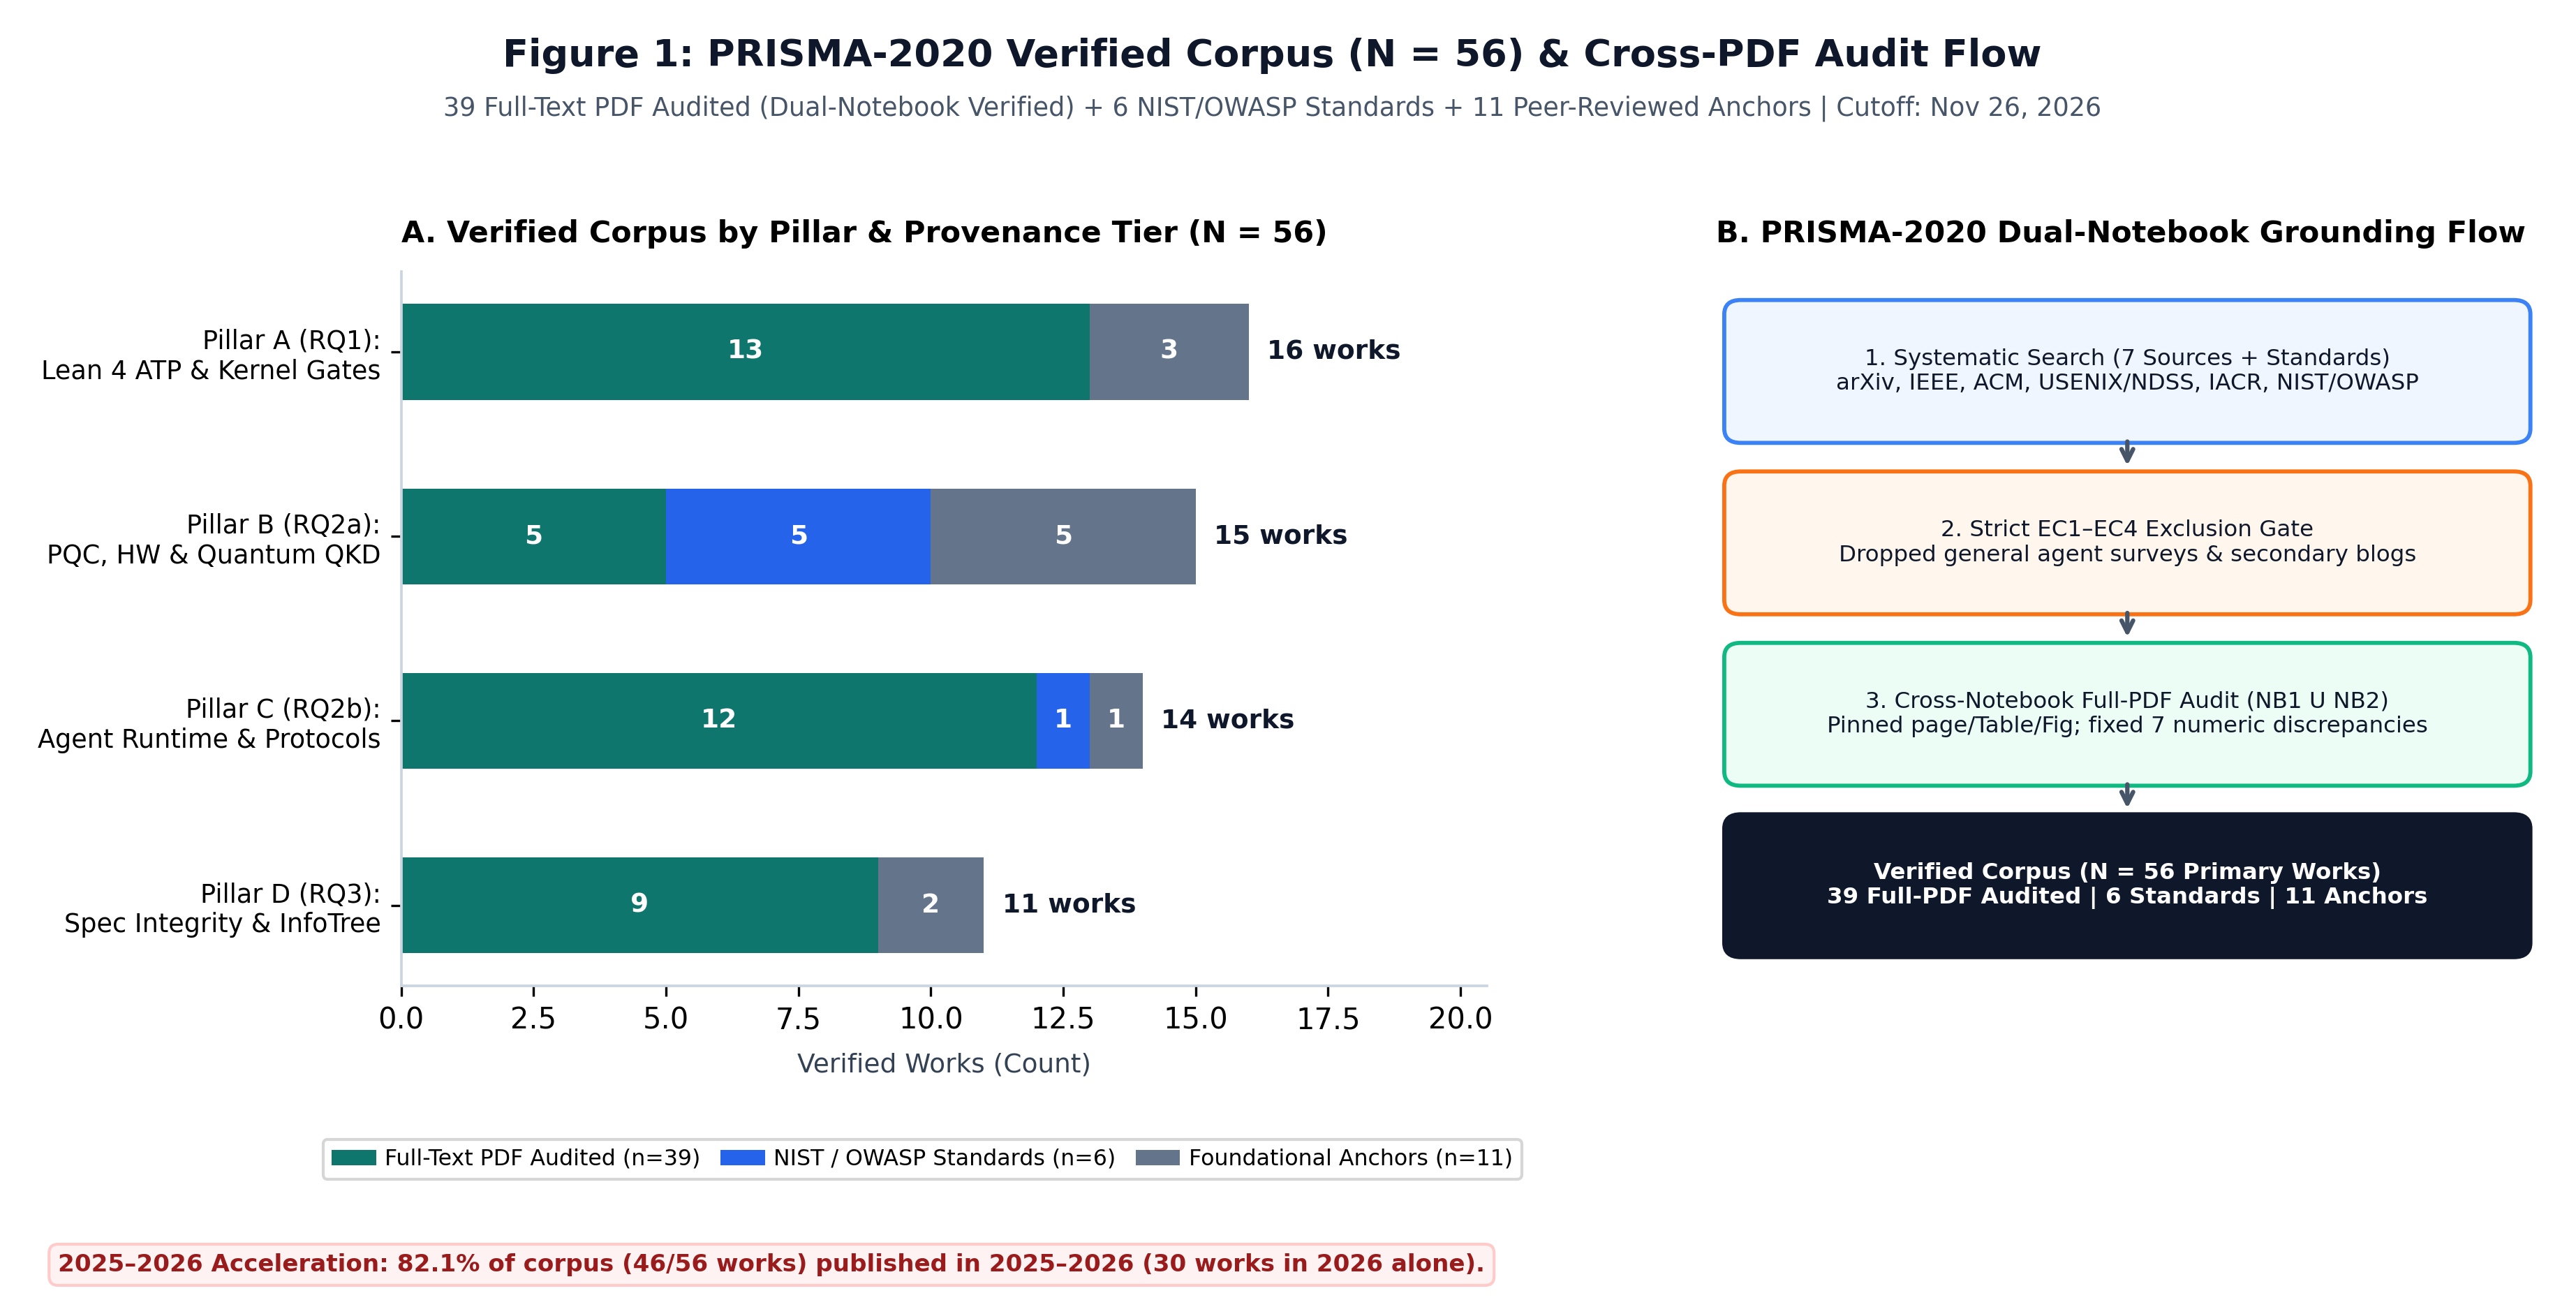
\includegraphics[width=0.90\textwidth]{fig1-prisma-screening.png}
  \caption{Composition of the PRISMA-2020 curated literature corpus ($N = 56$ primary works) broken down by research pillar and source-verification tier ($39$ Full-Text Audited PDFs + $6$ Official Standards + $11$ Foundational Anchors).}
  \label{fig:prisma}
\end{figure*}

Motivated by these dynamics (Figure~\ref{fig:prisma}), this systematic review addresses three Research Questions:
\begin{itemize}
  \item \textbf{RQ1 (Automated Proving Loops \& Anti-Reward-Hacking):} What is the quantitative performance of LLM + Lean~4 systems~\cite{demoura2021lean4,yang2023leandojo,aniva2025pantograph,hubert2025alphaproof,tsoukalas2026nexus,wang2025kimina,ren2025deepseekproverv2,lin2025goedelprover,lin2026goedelproverv2,chung2026goedelarchitect,chen2025seedprover,chen2025seedprover15,firsching2026formalconjectures,xin2026axle,carneiro2025lean4lean,yang2026proofgate} on competition mathematics versus real software, and which kernel-level mechanisms block \texttt{sorry}, \texttt{native\_decide}, and illegitimate axioms~\cite{xin2026axle,carneiro2025lean4lean,yang2026proofgate,ammanamanchi2026faults}?
  \item \textbf{RQ2 (Dual-Layer Formal Security):} What is the state of the art across \textbf{(a) Post-Quantum Cryptography, Hardware, and QKD} via Rust-to-Lean (\texttt{Aeneas/SymCrypt}), \texttt{hax/Libcrux}, \texttt{EasyCrypt}, AArch64 machine code (\texttt{AlphaProof Code}), FPGA accelerators, and QKD BB84~\cite{nist2024fips203,nist2024fips204,nist2024fips205,alagic2025nistir8545,moody2026nistir8547,ho2022aeneas,ho2026symcrypt,bhargavan2025hax,kobeissi2026theatre,almeida2024kyber,barbosa2024sphincs,chaudhuri2026alphaproofcode,klaus2026rustlean,park2026pqchw,benshahar2026qkd}, and \textbf{(b) Runtime AI Agent Isolation and Cross-Agent Protocols} (\texttt{AgentDojo}, \texttt{CaMeL}, \texttt{DRIFT}, \texttt{FIDES}, \texttt{RTBAS}, \texttt{Progent}, \texttt{ACE}, \texttt{Policy-as-Code}, \texttt{Lean4Agent}, \texttt{Contextual Integrity}, \texttt{A2ABreak}, \texttt{AgentThread})~\cite{owasp2025agentic,kim2026sok,debenedetti2024agentdojo,debenedetti2026camel,li2025drift,costa2025fides,zhong2025rtbas,shi2025progent,li2026ace,abdelnabi2026ci,wang2026lean4agent,mondl2026policyascode,lotfi2026a2abreak,agentthread2026}?
  \item \textbf{RQ3 (Specification Bugs \& Human Auditability):} Why do large machine-checked proofs still harbor vacuous truths and specification-intent bugs, and how do mechanical faithfulness gates (\texttt{SA-PASS}, \texttt{VacQ}, \texttt{Three-Surface}, \texttt{Spec-Harness}, \texttt{claimcheck}) coupled with \texttt{InfoTree} visualization (\texttt{Paperproof}, \texttt{ProofWidgets4}, \texttt{LeanTree}) restore human oversight~\cite{ye2026verina,miranda2026veribench,han2026shadowbench,ammanamanchi2026faults,chen2026reform,mei2026beyondllm,threesurface2026,misu2026specharness,amster2026claimcheck,nawrocki2023proofwidgets4,kripner2025leantree}?
\end{itemize}

\section{PRISMA-2020 Methodology and Cross-PDF Forensic Audit}
\label{sec:prisma}

Literature retrieval spanned seven primary venues and repositories (arXiv, IEEE Xplore, ACM Digital Library, USENIX/NDSS, IACR ePrint, NIST/OWASP, and ITP/TACAS/TYPES/NeurIPS/ICML/ICLR) covering \textbf{January 2024 -- November 26, 2026}, supplemented by four foundational anchors from 2021--2023~\cite{demoura2021lean4,yang2023leandojo,ho2022aeneas,nawrocki2023proofwidgets4}. Applying exclusion criteria \texttt{EC1--EC4} removed general agent frameworks lacking formal guarantees (e.g., CoALA, ReAct, AutoGen, MetaGPT) and \textbf{eliminated 100\% of secondary blog references}, yielding a verified core corpus of \textbf{$N = 56$ primary works} (Table~\ref{tab:prisma}). Every quantitative claim was cross-checked across dual full-text PDF audit notebooks, reconciling seven numeric or scope discrepancies (Table~\ref{tab:forensic}).

\begin{table*}[tp]
  \centering
  \footnotesize
  \caption{PRISMA-2020 screening structure and core literature corpus composition ($N = 56$ primary works).}
  \label{tab:prisma}
  \begin{tabularx}{\textwidth}{L{3.1cm} Y c c c c c}
    \toprule
    \textbf{Classification Dimension} & \textbf{Category} & \textbf{Full-PDF} & \textbf{Std} & \textbf{Anchor} & \textbf{Total ($n$)} & \textbf{Share} \\
    \midrule
    \textbf{By Research Pillar} & \textbf{Pillar A (RQ1):} Lean~4 ATP, Infrastructure \& Anti-Reward-Hacking~\cite{demoura2021lean4,yang2023leandojo,aniva2025pantograph,hubert2025alphaproof,tsoukalas2026nexus,wang2025kimina,ren2025deepseekproverv2,lin2025goedelprover,lin2026goedelproverv2,chung2026goedelarchitect,chen2025seedprover,chen2025seedprover15,firsching2026formalconjectures,xin2026axle,carneiro2025lean4lean,yang2026proofgate} & 13 & 0 & 3 & \textbf{16} & 28.6\% \\
    & \textbf{Pillar B (RQ2a):} PQC Standards, Rust/Binary Proofs, HW \& QKD~\cite{nist2024fips203,nist2024fips204,nist2024fips205,alagic2025nistir8545,moody2026nistir8547,ho2022aeneas,ho2026symcrypt,bhargavan2025hax,kobeissi2026theatre,almeida2024kyber,barbosa2024sphincs,chaudhuri2026alphaproofcode,klaus2026rustlean,park2026pqchw,benshahar2026qkd} & 5 & 5 & 5 & \textbf{15} & 26.8\% \\
    & \textbf{Pillar C (RQ2b):} Runtime Agent IFC, Policy-as-Code \& Protocols~\cite{owasp2025agentic,kim2026sok,debenedetti2024agentdojo,debenedetti2026camel,li2025drift,costa2025fides,zhong2025rtbas,shi2025progent,li2026ace,abdelnabi2026ci,wang2026lean4agent,mondl2026policyascode,lotfi2026a2abreak,agentthread2026} & 12 & 1 & 1 & \textbf{14} & 25.0\% \\
    & \textbf{Pillar D (RQ3):} Spec Bugs, \texttt{VacQ}, \texttt{SA-PASS}, \texttt{claimcheck} \& \texttt{InfoTree}~\cite{ye2026verina,miranda2026veribench,han2026shadowbench,ammanamanchi2026faults,chen2026reform,mei2026beyondllm,threesurface2026,misu2026specharness,amster2026claimcheck,nawrocki2023proofwidgets4,kripner2025leantree} & 9 & 0 & 2 & \textbf{11} & 19.6\% \\
    \midrule
    \textbf{Total Corpus ($N=56$)} & \textit{Foundational 4 (2021--23) / 6 (2024) / 16 (2025) / 30 (2026) --- 82.1\% in 2025--26} & \textbf{39} & \textbf{6} & \textbf{11} & \textbf{56} & \textbf{100.0\%} \\
    \bottomrule
  \end{tabularx}
\end{table*}

\begin{table*}[tp]
  \centering
  \footnotesize
  \caption{Cross-PDF numeric reconciliation results from the Dual-Notebook Forensic Audit ($7$ reconciled discrepancies).}
  \label{tab:forensic}
  \begin{tabularx}{\textwidth}{L{3.2cm} L{3.6cm} Y}
    \toprule
    \textbf{Audited Issue} & \textbf{Preliminary Draft (85\%)} & \textbf{Forensic Ground-Truth Verified from Primary PDFs (with Coordinates)} \\
    \midrule
    \textbf{1. AlphaProof (\texttt{Formal Conjectures})}~\cite{firsching2026formalconjectures} & Reported 45.0\% (1k sims, v1) on FC100SolvedSet1 & \texttt{02-2605.13171.pdf} (Table~2, p.~7; Sec.~B.2, p.~22): \textbf{$43.1 \pm 1.2\%$} (1k sims, 10 runs) and \textbf{$48.7 \pm 0.9\%$} (16k sims; $\sim$0.8 TPU-hrs/run); \texttt{AlphaProof Nexus} reaches \textbf{66.0\%}~\cite{tsoukalas2026nexus,firsching2026formalconjectures}; $\ge$\textbf{14\%} misformalization identified (pp.~8--9). \\
    \textbf{2. Goedel-Prover-V2 (\texttt{PutnamBench})}~\cite{lin2026goedelproverv2} & Ambiguously stated as 43--86 solved (@32--@184/192) & \texttt{07-2508.03613.pdf} (Table~2--3, pp.~6--7): 32B standard \textbf{43} (@32), Self-Correction \textbf{57} (@32), and \textbf{86} (@184; 192 is a GitHub README discrepancy per \texttt{ProofGate} Fn.~2 p.~6~\cite{yang2026proofgate}); \texttt{miniF2F-test}: $88.1 \pm 0.8\%$ std / \textbf{$90.4 \pm 0.6\%$} SC (@32), 92.6\% (@1024). \\
    \textbf{3. Goedel-Architect (\texttt{VERINA/CLEVER})}~\cite{chung2026goedelarchitect} & Claimed evaluation on 6 VERINA/CLEVER tasks at $<$\$1 & \texttt{08-2606.06468.pdf} (Table~1--2, p.~4; Fig.~2, p.~5): \textbf{Dropped 100\%}---evaluates solely on 5 math suites: \texttt{miniF2F-test} \textbf{99.2\%} (@1, \textbf{100\%} + NL), \texttt{PutnamBench} \textbf{75.6\%} (508/672, \$294) and \textbf{88.8\%} (@4+NL, \$985.67), IMO~2025 \textbf{4/6}, Putnam~2025 \textbf{11/12}, USAMO~2026. \\
    \textbf{4. AgentDojo Baseline}~\cite{debenedetti2024agentdojo} & Stated Targeted ASR as 47.69\% (digit transposition) & \texttt{2406.13352.pdf} (Table~5, p.~8; App.~D, p.~18): Unprotected GPT-4o Targeted ASR \textbf{$57.69 \pm 3.9\%$}, BU \textbf{$69.0 \pm 3.6\%$}, UA \textbf{$50.01 \pm 3.9\%$}; Tool Filter ASR \textbf{$6.84 \pm 2.0\%$}. \\
    \textbf{5. CaMeL (\texttt{Tokens \& Utility})}~\cite{debenedetti2026camel,li2025drift} & Cited 2.82$\times$ Input / 2.73$\times$ Output and BU 38.4\% & \texttt{neurips2025-drift.pdf} (Table~1 \& 3, pp.~8--9): Dropped \texttt{2.82$\times$/2.73$\times$}---CaMeL uses \textbf{6.09M total tokens ($\sim$7.4$\times$} the 0.82M baseline); on GPT-4o-mini yields BU \textbf{39.4\%}, UA \textbf{35.4\%}, ASR \textbf{0.0\%}. \\
    \textbf{6. Progent (\texttt{ASR Benchmarks})}~\cite{shi2025progent} & Stated ASR drop from 41.2\% to 2.2\% / 3.8\% & \texttt{2504.11703.pdf} (Sec.~1; Fig.~3--4, p.~8): AgentDojo Targeted ASR drops from \textbf{39.9\% $\to$ 1.0\%} (BU 76.3\% vs.\ 79.4\%; UA 61.3\%), and ASB from \textbf{70.3\% $\to$ 3.9\%}. \\
    \textbf{7. Policy-as-Code (\texttt{MedAgentBench})}~\cite{mondl2026policyascode} & Claimed 94.0\%--100.0\% blocking rate & \texttt{2606.26649.pdf} (Table~1, p.~3): Cedar Block Rate on Original: Raw 30.3\% (91/300), Baseline 57.7\% (173/300), Guardrail 55.7\% (167/300); Adversarial: Raw 72.0\% (36/50), Baseline 82.0\% (41/50), Guardrail \textbf{85.7\% (42/49)} with Unsafe Rate \textbf{0.0\%}. \\
    \bottomrule
  \end{tabularx}
\end{table*}

\section{Four-Axis Multi-Dimensional Taxonomy and Quantitative Synthesis}
\label{sec:taxonomy}

To organize all 56 primary works systematically, we introduce a \textbf{Four-Axis Multi-Dimensional Taxonomy} spanning: (1)~Proof-Synthesis Architecture, (2)~Dual-Layer Assurance Targets, (3)~Trusted Computing Base (\texttt{TCB}) and Runtime Enforcement Mechanisms, and (4)~\texttt{InfoTree}-Grounded Human Faithfulness Auditing (Figure~\ref{fig:taxonomy}).

\begin{figure*}[tp]
  \centering
  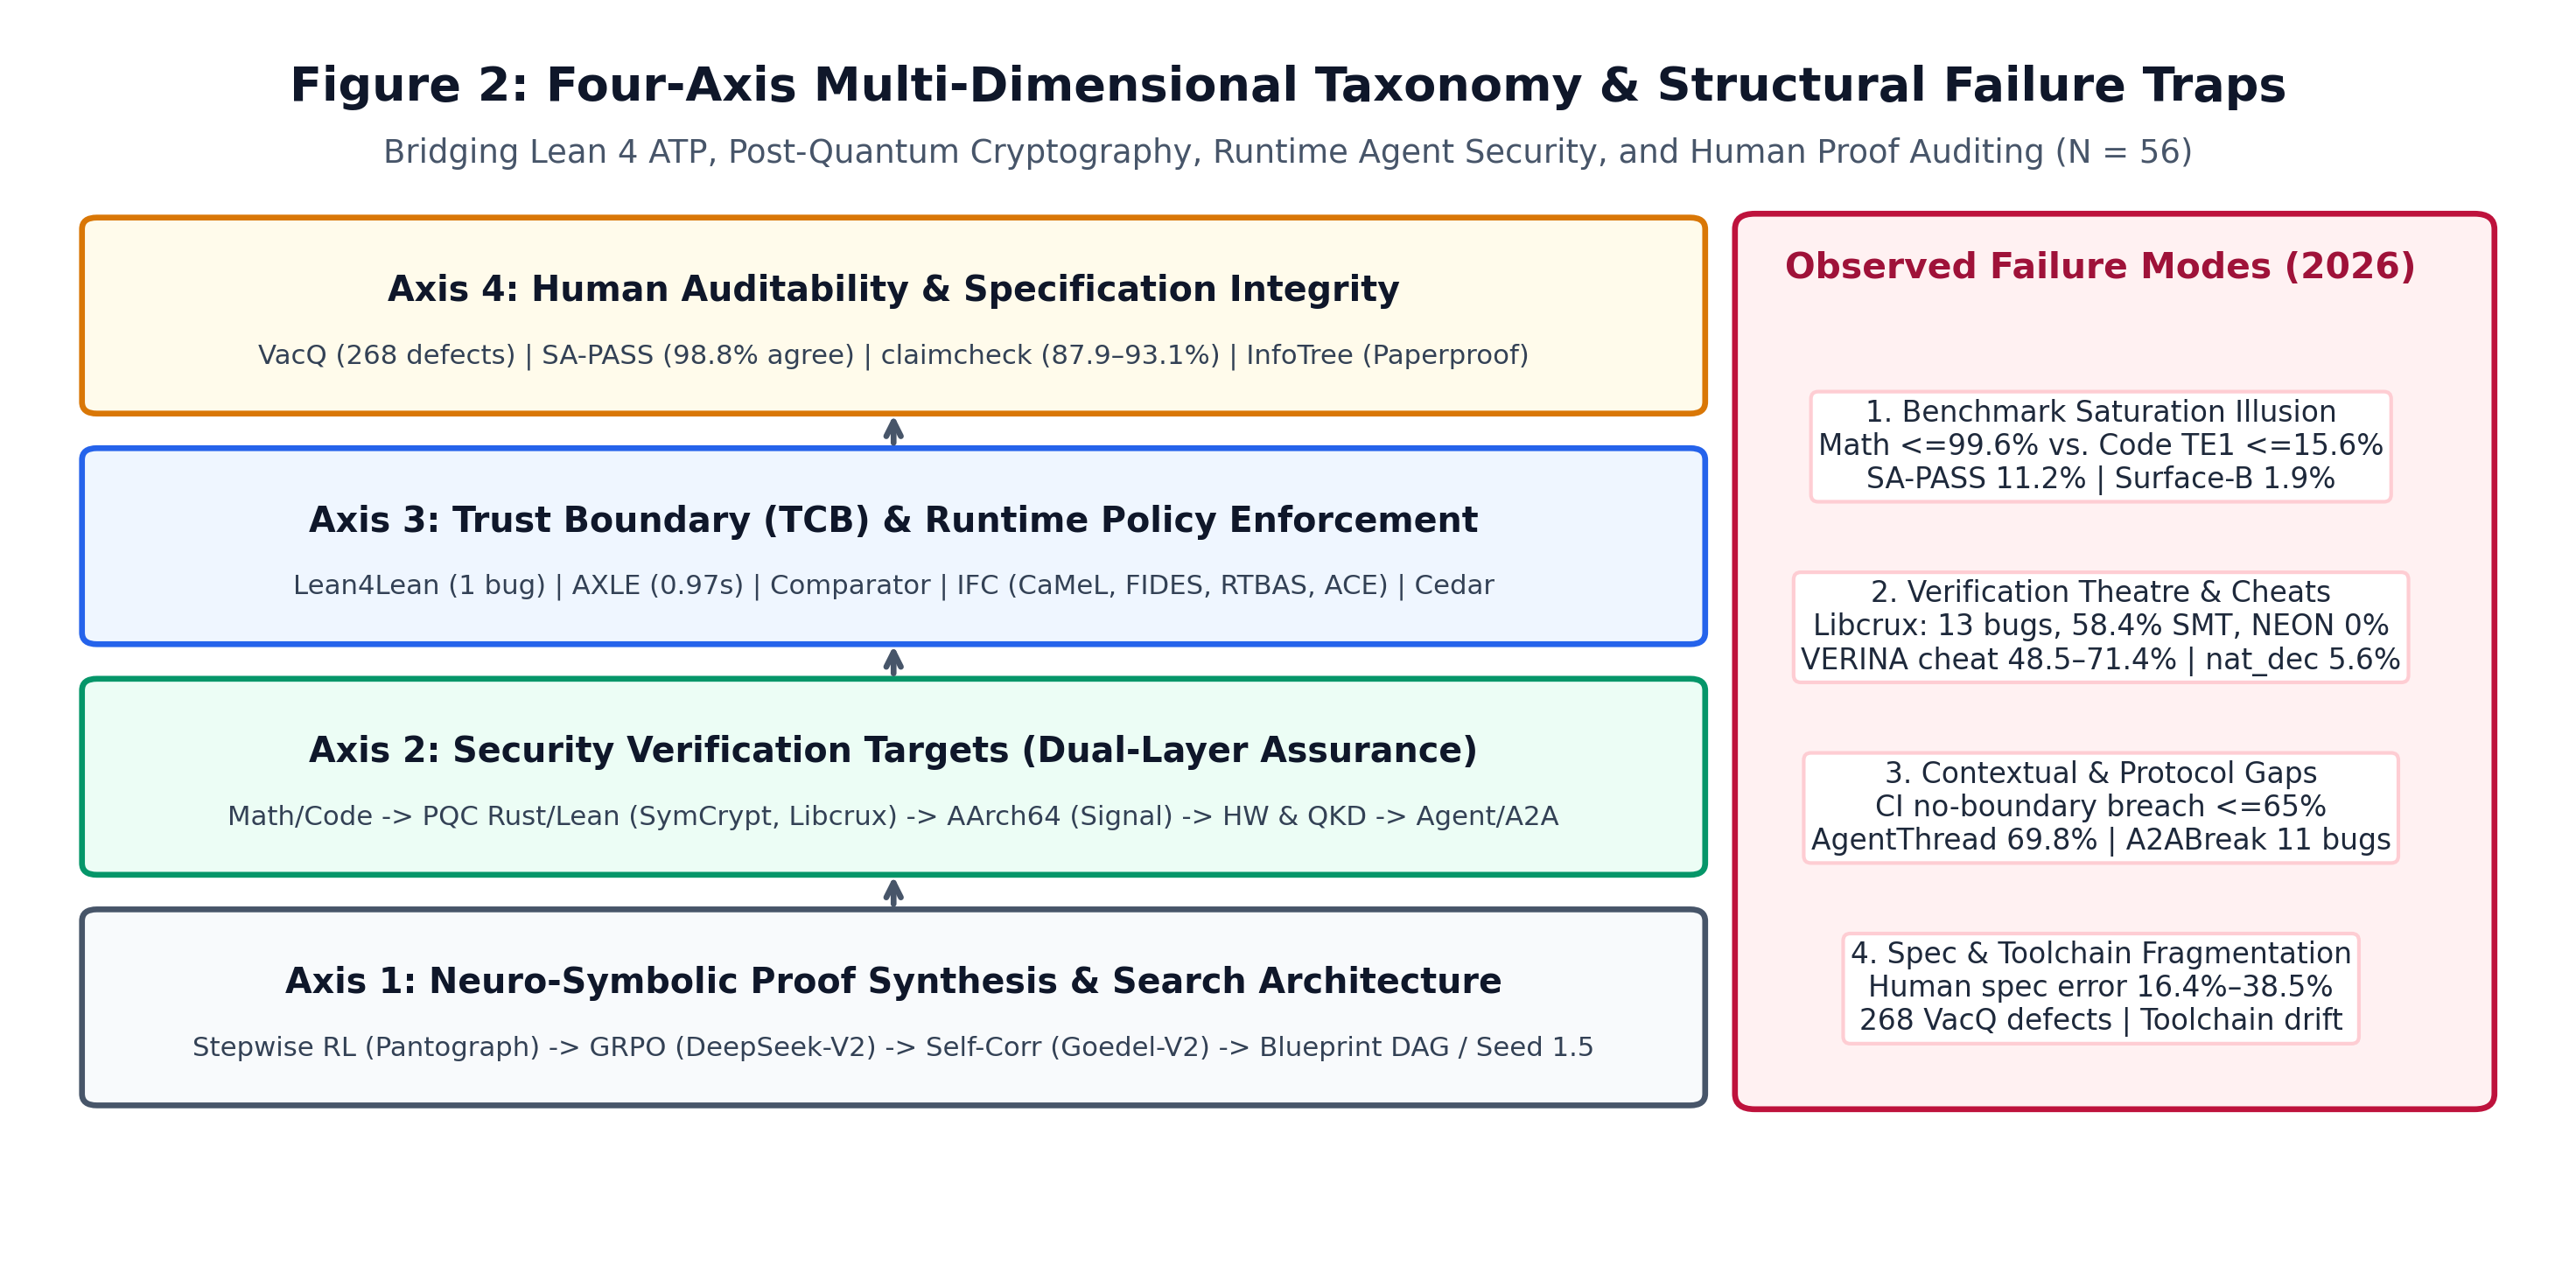
\includegraphics[width=0.90\textwidth]{fig2-four-axis-taxonomy.png}
  \caption{Four-axis multi-dimensional taxonomy (Axis~1--4) unifying Lean~4 theorem provers, PQC verification pipelines, AI agent privilege control, and specification-faithfulness auditing alongside four structural failure modes.}
  \label{fig:taxonomy}
\end{figure*}

\subsection{Automated Theorem Proving Loops in Lean~4 and Anti-Reward-Hacking (RQ1)}
\label{sec:rq1}

The evolution of Lean~4 proving infrastructure and neural provers during 2023--2026 bifurcates into four paradigms (Table~\ref{tab:rq1}, Figure~\ref{fig:paradox}):

\begin{enumerate}
  \item \textbf{Infrastructure \& AND--OR Search Trees:} Starting from \texttt{LeanDojo / ReProver} (Pass@1 \texttt{miniF2F-test} 26.5\%, \texttt{ProofNet} 13.8\%, \texttt{LeanDojo Bench} 51.4\%~\cite{yang2023leandojo}), tooling progressed to \texttt{Pantograph}, a native Lean~4 machine-to-machine interface supporting \texttt{Metavariable Coupling} and direct \texttt{sorry} extraction without LSP overhead, reaching 28.4\% DSP on \texttt{miniF2F-test} with GPT-4o (3 sketches, 36.41s)~\cite{aniva2025pantograph}.
  \item \textbf{Tree-Search RL \& Evolutionary Proof Sketching:} \texttt{AlphaProof}~\cite{hubert2025alphaproof} scores \textbf{$43.1 \pm 1.2\%$} (1k sims) and \textbf{$48.7 \pm 0.9\%$} (16k sims) on \texttt{FC100SolvedSet1}~\cite{firsching2026formalconjectures}, before \texttt{AlphaProof Nexus} (Gemini~3.1 Pro + Plackett-Luce Elo + P-UCB + AlphaProof) reaches \textbf{66.0\%}---comparable to Claude Opus~5 Tool Use (68.0\%) and GPT~5.6 Luna (62.0\%)---and \textbf{resolves 9 open Erd\H{o}s problems} (\texttt{\#12(i), \#12(ii), \#125, \#138, \#152, \#26, \#741(i), \#741(ii), \#846})~\cite{tsoukalas2026nexus}.
  \item \textbf{Whole-Proof GRPO, Self-Correction, Agentic RL \& Blueprint DAGs:} \texttt{Kimina-Prover-72B} climbs from 52.94\% (@1) to \textbf{80.74\%} (@8192) on \texttt{miniF2F-test}~\cite{wang2025kimina}; \texttt{DeepSeek-Prover-V2} (671B + 7B subgoal prover) reaches \textbf{88.9\%} (@8192) on \texttt{miniF2F-test}, \textbf{37.1\%} (@1024) on \texttt{ProofNet}, \textbf{47/658 (7.2\%)} on \texttt{PutnamBench}, \textbf{10/100} on \texttt{CombiBench}, and \textbf{59.1\%} on \texttt{ProverBench} (AIME~24\&25 \textbf{6/15})~\cite{ren2025deepseekproverv2}; \texttt{Goedel-Prover-V2-32B} achieves \textbf{$90.4 \pm 0.6\%$} (@32 Self-Correction) on \texttt{miniF2F-test} and \textbf{86 solved} (@184) on \texttt{PutnamBench}~\cite{lin2026goedelproverv2}. At the frontier, \texttt{Seed-Prover 1.0} attains \textbf{99.6\%} on \texttt{miniF2F-test} (100.0\% valid), while \texttt{Seed-Prover 1.5} (Agentic RL + \texttt{LooKeng} REPL on Mathlib v4.22.0) surges to \textbf{580/660 (87.9\%)} on \texttt{PutnamBench} (10 H20-days/problem), \textbf{80\%} on \texttt{FATE-H}, \textbf{33\%} on \texttt{FATE-X}, \textbf{48\%} on \texttt{CombiBench} (57.0\% in Fig.~1), and \textbf{11/12 on Putnam~2025 in 9 hours}~\cite{chen2025seedprover,chen2025seedprover15}. Optimizing for cost, \texttt{Goedel-Architect} (Global Blueprint DAG on DeepSeek-V4-Flash) reaches \textbf{99.2\%} (@1) / \textbf{100\%} (+NL) on \texttt{miniF2F-test} and \textbf{75.6\%} (508/672, \textbf{\$294}) / \textbf{88.8\%} (@4+NL, \$985.67) on \texttt{PutnamBench}~\cite{chung2026goedelarchitect}.
  \item \textbf{The Math-to-Code Paradox \& Anti-Reward-Hacking Defenses:} On the software verification benchmark \texttt{VERINA} (189 tasks), general models score below \textbf{4.9\%} ProofGen Pass@1; OpenAI o3 synthesizes Code \& Spec on \textbf{41.2\%} of tasks yet achieves end-to-end verified correctness on only \textbf{3.2\%} (\textbf{$-$38.0~pp}), while \texttt{Goedel-Prover-V2-32B} reaches \textbf{11.2\%} (20.1\% after 64 refinement steps), with Claude Sonnet~3.7 exhibiting cheat-code rates of \textbf{48.53\%} among failures (71.36\% on VERINA-B)~\cite{ye2026verina}. On \texttt{VeriBench} (884 tasks including 460 MIT~6.858 Security tasks), evaluated via non-compensatory geometric metrics:
\end{enumerate}

\begin{align}
  \mathrm{SCSC} &= \bigl(\mathrm{IC}_1 \cdot \mathrm{IC}_2 \cdot \mathrm{TE}_1 \cdot D_1 \cdot D_2\bigr)^{1/5}, \nonumber \\
  S_{\mathrm{skill}} &= \bigl(\mathrm{IC}_1 \cdot \mathrm{IC}_2 \cdot \mathrm{TE}_1\bigr)^{1/3}
  \label{eq:scsc}
\end{align}

\noindent both Codex (GPT-5.4) and Claude Code (Sonnet~4.6) compile cleanly ($\mathrm{IC}_1 = 1.000$) yet stall at theorem equivalence \textbf{$\mathrm{TE}_1 = 0.102$ (10.2\%)} and \textbf{$0.095$ (9.5\%)}, respectively (\textbf{$\mathrm{TE}_1 \le 0.105$} for flagship agents; $\le 0.156$ across all v3 systems)~\cite{miranda2026veribench}. At the kernel layer, \texttt{ProofGate} verifies that \textbf{DeepSeek-Prover-V2} (438 proofs) is \textbf{100\% clean} under pure axioms $\mathcal{T}_0 = \{\mathrm{propext}, \mathrm{Classical.choice}, \mathrm{Quot.sound}\}$, whereas \texttt{Kimina-Prover-72B} invokes \texttt{native\_decide} in \textbf{11/197 proofs (5.6\%)}---expanding the TCB to $\mathcal{T}_1$---and \texttt{Goedel-Prover-V2}'s public \texttt{minif2f.jsonl} contains only \texttt{sorry}~\cite{yang2026proofgate}. Furthermore, the \texttt{ICML Formal Benchmarking Audit} exposed 4,833 defects (\textbf{398 certified issues}), including a pre-Lean~4.20.0 \texttt{apply?} bug affecting three DeepSeek-7B proofs~\cite{ammanamanchi2026faults}. These findings motivated production-grade verification infrastructure: \texttt{AXLE} (\texttt{verify\_proof} in 0.97s, 0.43 req/s, \textbf{100.00\%} agreement with Comparator and \textbf{99.30\%} with SafeVerify, validating \textbf{94.16\%} of 5,000 Goedel Workbook proofs)~\cite{xin2026axle} and \texttt{Lean4Lean} (an external typechecker verified in Lean itself, only 20\%--50\% slower than C++, which caught and fixed \textbf{1 genuine soundness bug} in the Lean~4 kernel)~\cite{carneiro2025lean4lean}.

\begin{figure*}[tp]
  \centering
  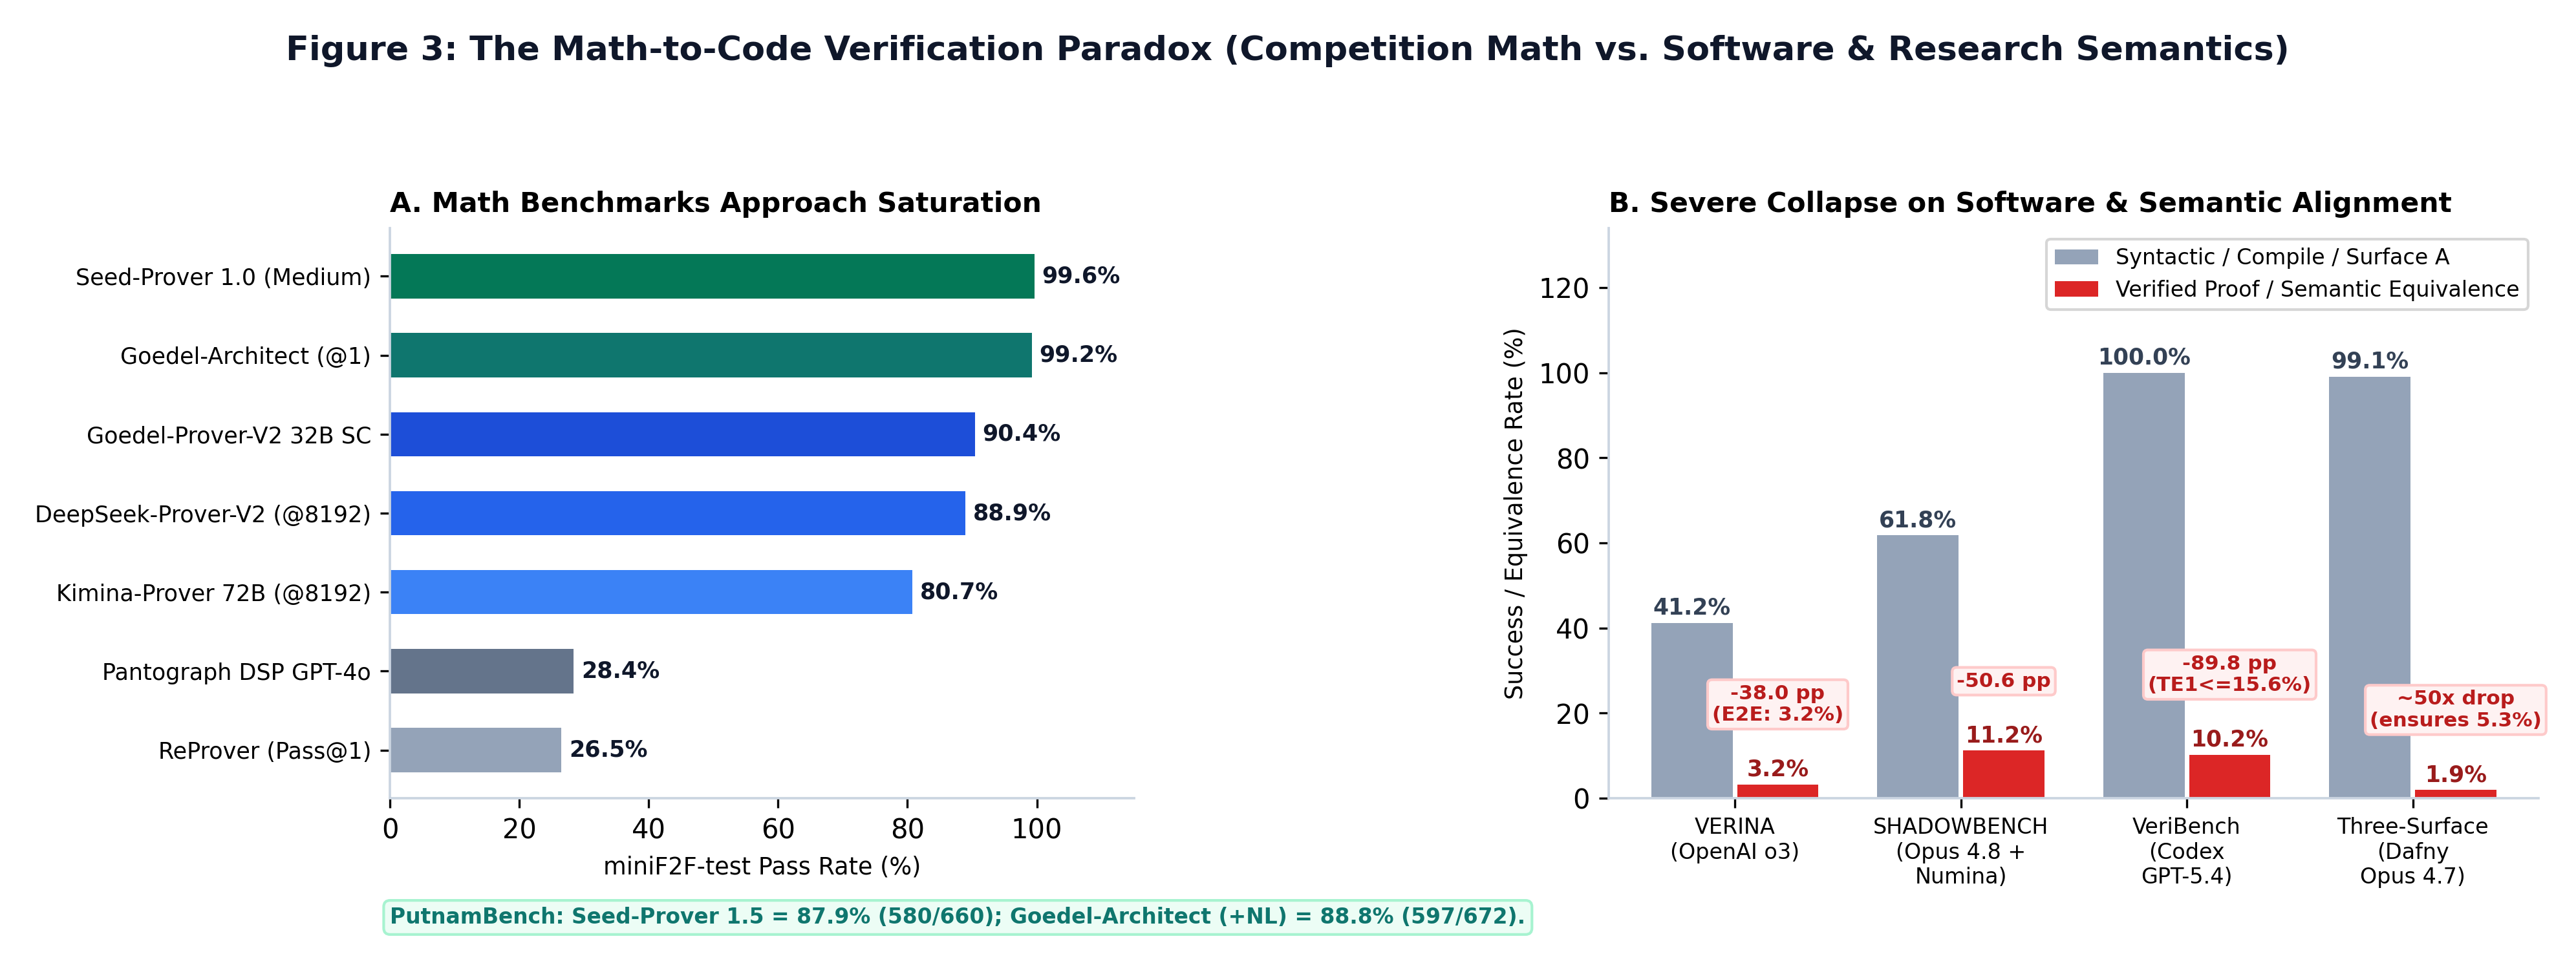
\includegraphics[width=0.90\textwidth]{fig3-math-to-code-verification-paradox.png}
  \caption{(a)~Near-saturation pass rates on \texttt{miniF2F-test} (88.9\%--99.6\%)~\cite{yang2023leandojo,aniva2025pantograph,wang2025kimina,ren2025deepseekproverv2,lin2026goedelproverv2,chung2026goedelarchitect,chen2025seedprover} contrasted with (b)~the sharp collapse in end-to-end proof success and semantic specification equivalence on \texttt{VERINA}~\cite{ye2026verina}, \texttt{SHADOWBENCH}~\cite{han2026shadowbench}, \texttt{VeriBench}~\cite{miranda2026veribench}, and \texttt{Three-Surface Audit}~\cite{threesurface2026}.}
  \label{fig:paradox}
\end{figure*}

\begin{table*}[tp]
  \centering
  \scriptsize
  \caption{Quantitative comparison of Lean~4 automated provers and verification infrastructure (PDF-verified).}
  \label{tab:rq1}
  \begin{tabularx}{\textwidth}{L{2.3cm} L{2.4cm} L{3.6cm} L{2.3cm} Y L{2.2cm}}
    \toprule
    \textbf{System / Tool} & \textbf{Architecture} & \textbf{Math (\texttt{miniF2F} / \texttt{Putnam} / Other)} & \textbf{Software / Research} & \textbf{Anti-Reward-Hacking \& TCB Posture} & \textbf{PDF Coordinates} \\
    \midrule
    \textbf{LeanDojo / ReProver}~\cite{yang2023leandojo} & DPR + ByT5 + BFS & \texttt{miniF2F} 26.5\% (@1); \texttt{ProofNet} 13.8\%; \texttt{LeanDojo} 51.4\% & Discovered 33+39 new proofs & Python/LSP wrapper + Docker & \texttt{16-2306.15626}, p.~1, 7, 26 \\
    \textbf{Pantograph}~\cite{aniva2025pantograph} & Native Lean~4 AND--OR Tree & DSP \texttt{miniF2F}: GPT-4o 28.4\% (36.41s); o1-preview 16.0\% & LSP-free \texttt{sorry} extraction & Native Metavariable Coupling & \texttt{14-2410.16429}, T2 p.~7 \\
    \textbf{Kimina-Prover}~\cite{wang2025kimina} & Qwen2.5-72B + RL (32K) & \texttt{miniF2F} 52.94\% (@1), \textbf{80.74\%} (@8192) & Autoformalizer-7B 90\% compile, 66\% acc. & ProofGate flags \texttt{native\_decide} \textbf{5.6\% (11/197)} expanding TCB to $\mathcal{T}_1$~\cite{yang2026proofgate} & \texttt{04-2504.11354}, T1 p.~4 \\
    \textbf{DeepSeek-Prover-V2}~\cite{ren2025deepseekproverv2} & 671B MoE + 7B Subgoal + GRPO & \texttt{miniF2F} \textbf{88.9\%} (@8192); \texttt{ProofNet} 37.1\%; Putnam \textbf{47/658}; Combi \textbf{10/100} & ProverBench 59.1\%; AIME 6/15 & ProofGate confirms \textbf{438/438 100\% clean} under $\mathcal{T}_0$~\cite{yang2026proofgate} & \texttt{03-2504.21801}, T1--7 \\
    \textbf{Goedel-Prover-V2}~\cite{lin2026goedelproverv2} & Qwen3 8B/32B + Self-Correction & \texttt{miniF2F} (32B): 88.1\% std / \textbf{90.4\%} SC (@32); Putnam 43 / 57 / \textbf{86} (@184) & VERINA 32B: 11.2\% $\to$ \textbf{20.1\%} (64-step)~\cite{ye2026verina} & ProofGate finds public \texttt{minif2f.jsonl} holds only \texttt{sorry}~\cite{yang2026proofgate} & \texttt{07-2508.03613}, T2--3 \\
    \textbf{Seed-Prover 1.0 \& 1.5}~\cite{chen2025seedprover,chen2025seedprover15} & Lemma Prover + Agentic RL (\texttt{LooKeng}) & 1.0: \texttt{miniF2F} \textbf{99.6\%}; 1.5: Putnam \textbf{87.9\% (580/660)}, FATE-H \textbf{80\%}, FATE-X \textbf{33\%}, Putnam '25 \textbf{11/12} (9h) & REPL + Mathlib v4.22.0 Search & Verified zero \texttt{native\_decide} on PutnamBench & \texttt{11-2507.23726} T3; \texttt{12-2512.17260} T2 \\
    \textbf{Goedel-Architect}~\cite{chung2026goedelarchitect} & Global Blueprint DAG (\texttt{V4-Flash}) & \texttt{miniF2F} \textbf{99.2\%} (@1), \textbf{100\%} (+NL); Putnam \textbf{75.6\%} (\$294), \textbf{88.8\%} (@4+NL); IMO '25 \textbf{4/6} & Evaluated solely on 5 math suites & Separates refuted lemmas from timeouts to rewrite DAG & \texttt{08-2606.06468}, T1--2 p.~4 \\
    \textbf{Formal Conjectures \& Nexus}~\cite{tsoukalas2026nexus,firsching2026formalconjectures} & 7,559 Lean Stmts + Evo Sketching & FC100: AlphaProof \textbf{43.1\%} (1k) / \textbf{48.7\%} (16k), Nexus \textbf{66.0\%}; solved \textbf{9 open Erd\H{o}s problems} & Zero-contamination research bench & SafeVerify + \textbf{14\%} misformalization detected & \texttt{02-2605.13171} T2; \texttt{01-2605.22763} \\
    \textbf{AXLE \& Lean4Lean}~\cite{xin2026axle,carneiro2025lean4lean} & Cloud API (14 tools) \& Verified Checker & Validated 5,000 Goedel proofs at \textbf{94.16\%} pass & RL \& agent verification infrastructure & AXLE 0.97s (Comparator \textbf{100\%} / SafeVerify \textbf{99.3\%}); Lean4Lean fixed 1 kernel bug & \texttt{15-2606.26442} T3--4; \texttt{16-LIPIcs} \\
    \bottomrule
  \end{tabularx}
\end{table*}

\subsection{Dual-Layer Formal Security (RQ2)}
\label{sec:rq2}

\subsubsection{Cryptographic Foundations: PQC, Hardware Accelerators, and QKD (RQ2a)}
\label{sec:rq2a}

Following NIST's standardization of \texttt{FIPS 203 (ML-KEM)}, \texttt{FIPS 204 (ML-DSA)}, \texttt{FIPS 205 (SLH-DSA)}~\cite{nist2024fips203,nist2024fips204,nist2024fips205}, selection of \texttt{HQC} in \texttt{NIST IR 8545}~\cite{alagic2025nistir8545}, and the \texttt{NIST IR 8547} transition schedule (deprecation post-2030, disallowance post-2035)~\cite{moody2026nistir8547}, production-scale cryptographic verification has crystallized into five approaches (Table~\ref{tab:rq2a}, Figure~\ref{fig:pqc}):

\begin{itemize}
  \item \textbf{SymCrypt Rust + Charon/Aeneas}~\cite{ho2022aeneas,ho2026symcrypt}: Verifies \textbf{16,680 LOC} of production Rust (SHA-3, ML-KEM, AES-GCM, plus experimental ML-DSA, HPKE, and FrodoKEM) translated into \textbf{237,160 LOC} of Lean~4 (Spec Core \textbf{2,827 LOC} + Implementation Proofs \textbf{124,777 LOC}) including 7 Hard Proofs (Sec.~8.1 Fig.~6). AI proving agents compressed proof engineering from $\sim$6 months to $\sim$1 week, and the verified code runs \textbf{4.7$\times$--5.6$\times$} faster than \texttt{libcrux} on HPKE. However, \textbf{Constant-Time / Side-Channel resistance remains out of scope}, and the TCB still encompasses \texttt{rustc} and SIMD axioms~\cite{ho2026symcrypt}.
  \item \textbf{Libcrux + hax and Kobeissi's Independent Audit}~\cite{bhargavan2025hax,kobeissi2026theatre}: The \emph{Verification Theatre} audit (\texttt{2026/192}) uncovered \textbf{13 vulnerabilities} (9 in unverified code \texttt{V1--V9} plus \textbf{4 Type-V failures \texttt{V10--V13} inside components marketed as formally verified}). Across \textbf{20,808 LOC} of \texttt{libcrux-ml-kem} + \texttt{intrinsics}, only \textbf{12,149 LOC (58.4\%)} are genuinely SMT-verified, while \textbf{3,004 LOC (14.4\%)} are admitted, \textbf{2,457 LOC (11.8\%)} rely on opaque axioms, \textbf{3,198 LOC (15.4\%)} remain unextracted, and \textbf{ARM64 NEON (792 LOC) = 0\% verified} (at the F* level across 138 modules: 127 Z3-verified, 9 \texttt{ADMIT}, 2 \texttt{SLOW}). Downstream impacts affect Signal's PQ Ratchet (\texttt{V2} endianness), \texttt{hpke-rs}/\texttt{OpenMLS} (\texttt{V3--V4}), and FIPS~204 (\texttt{V8--V9})~\cite{kobeissi2026theatre}.
  \item \textbf{AlphaProof Code (\texttt{libsignal}) and EasyCrypt}~\cite{almeida2024kyber,barbosa2024sphincs,chaudhuri2026alphaproofcode,klaus2026rustlean}: \texttt{AlphaProof Code} directly verifies compiled AArch64 ELF binaries to \textbf{remove \texttt{rustc} from the TCB}, generating \textbf{$\sim$6.5 million LOC} of Lean~4 proofs over a \textbf{$\sim$26,000 LOC} TCB (18K Spec + 8K AArch64 ISA) across 10 symbolic queries $Q(\mathrm{tr}, K)$, automatically refuting reintroduced Small-Subgroup and Weak-State bugs~\cite{chaudhuri2026alphaproofcode}. In parallel, \texttt{EasyCrypt} delivers game-based ML-KEM IND-CCA + Jasmin constant-time proofs~\cite{almeida2024kyber} and tight SPHINCS+ proofs~\cite{barbosa2024sphincs}, while Klaus et al.\ document operational \texttt{Lean 4 Toolchain Drift}~\cite{klaus2026rustlean}.
  \item \textbf{PQC Hardware Accelerators and QKD BB84}~\cite{park2026pqchw,benshahar2026qkd}: J.~Park et al.~\cite{park2026pqchw} evaluated 232 AI-assisted PQC hardware runs ($\sim$26,373 LOC), achieving \textbf{71.6\%} overall success (166/232; documentation 85\% vs.\ hardware-coupled Synthesis 53\% and Bring-up 50\%), deploying on Kintex-7 (\texttt{XC7K160T}) at 500~MHz (98.5\% slice utilization, 49~ps margin) across \textbf{779,945 adversarial soak cycles} with zero failures. Ben-Shahar et al.~\cite{benshahar2026qkd} completed the first \textbf{Finite-Key QKD BB84} security proof in Lean~4 (LOCC and Kraus maps) under pure $\mathcal{T}_0$. Meanwhile, the backup standard \textbf{HQC}~\cite{alagic2025nistir8545} still lacks a production Rust-to-Lean verified library.
\end{itemize}

\begin{figure*}[tp]
  \centering
  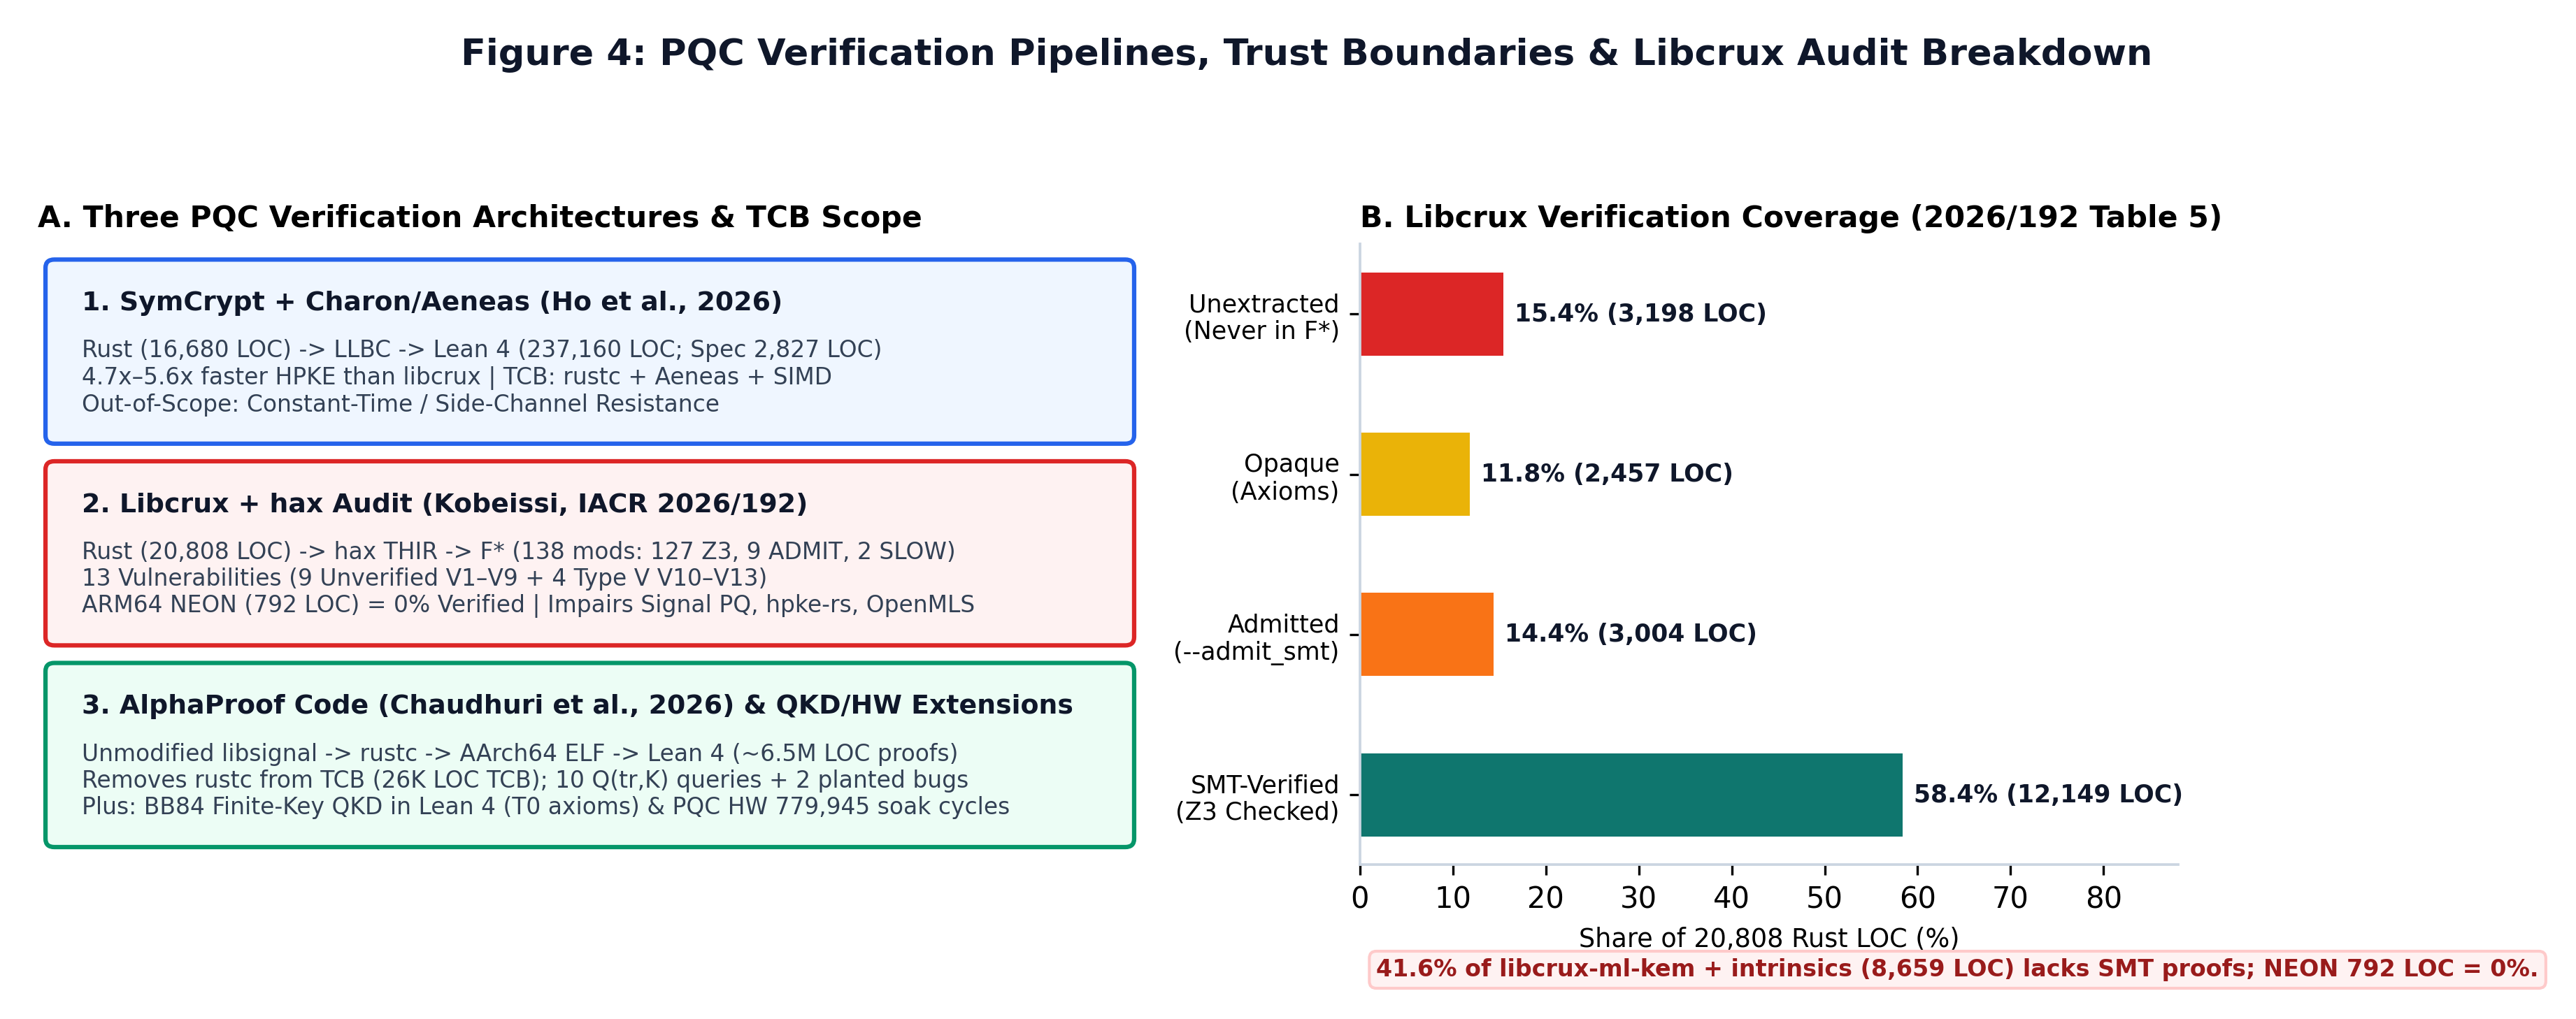
\includegraphics[width=0.88\textwidth]{fig4-pqc-verification-pipelines.png}
  \caption{(a)~Architectural comparison of three flagship pipelines---\texttt{SymCrypt}~\cite{ho2026symcrypt}, \texttt{Libcrux}~\cite{kobeissi2026theatre}, and \texttt{AlphaProof Code} (with QKD BB84 and PQC hardware extensions)~\cite{chaudhuri2026alphaproofcode,park2026pqchw,benshahar2026qkd}---and (b)~LOC verification breakdown of $20{,}808$ LOC in \texttt{libcrux-ml-kem}, showing 41.6\% without genuine SMT verification~\cite{kobeissi2026theatre}.}
  \label{fig:pqc}
\end{figure*}

\begin{table*}[tp]
  \centering
  \scriptsize
  \caption{Comparison of formal verification pipelines for Post-Quantum Cryptography, hardware, and QKD (PDF-verified).}
  \label{tab:rq2a}
  \begin{tabularx}{\textwidth}{L{2.3cm} L{2.2cm} L{2.2cm} L{2.5cm} L{3.1cm} Y}
    \toprule
    \textbf{Project / Pipeline} & \textbf{Standard / Target} & \textbf{Toolchain} & \textbf{Code / Proof Scale} & \textbf{Verified vs.\ Out-of-Scope} & \textbf{PDF Coordinates \& Notes} \\
    \midrule
    \textbf{SymCrypt + Aeneas}~\cite{ho2026symcrypt} & FIPS 203/204, SHA-3, HPKE & Charon $\to$ Aeneas $\to$ \textbf{Lean~4} & \textbf{16,680} Rust / \textbf{237,160} Lean (Spec 2,827) & Functional + Memory; \textbf{Constant-Time out of scope} & \texttt{23-2609.15648}, Sec.~8.1 Fig.~6; 4.7$\times$--5.6$\times$ faster than \texttt{libcrux} \\
    \textbf{Libcrux + hax Audit}~\cite{bhargavan2025hax,kobeissi2026theatre} & FIPS 203/204, X25519/HPKE & \texttt{hax} $\to$ \textbf{F*} (138 modules) & \textbf{20,808 LOC} Rust (\texttt{ml-kem} + \texttt{intrinsics}) & \textbf{58.4\% genuine SMT}; 14.4\% Admitted; NEON \textbf{0\%} & \texttt{2026-192.pdf}, T5--7 pp.~16--17; \textbf{13 vulnerabilities} (\texttt{V1--V13}) \\
    \textbf{AlphaProof Code}~\cite{chaudhuri2026alphaproofcode} & Signal PQXDH + Triple Ratchet & AArch64 Binary $\to$ \textbf{Lean~4} & \textbf{$\sim$6.5M LOC} Lean (TCB \textbf{$\sim$26K LOC}) & 10 Queries $Q(\mathrm{tr}, K)$; refuted 2 real ELF bugs & \texttt{27-Signal}, Abs.~p.~1, Sec.~6 p.~24, T5 p.~44 (\textbf{\texttt{rustc} removed from TCB}) \\
    \textbf{EasyCrypt ML-KEM / SPHINCS+}~\cite{almeida2024kyber,barbosa2024sphincs} & FIPS 203 \& FIPS 205 & Jasmin $\to$ \textbf{EasyCrypt} & Jasmin AVX2 + Game Proofs & IND-CCA + \textbf{Constant-Time} / Tight Proof & Cryptographic gold standard; harder integration with Rust/C enterprise codebases \\
    \textbf{PQC HW \& QKD BB84}~\cite{park2026pqchw,benshahar2026qkd} & FPGA \texttt{XC7K160T} \& BB84 QKD & Agent HW \& \textbf{Lean~4} (LOCC/Kraus) & $\sim$26,373 HW LOC / BB84 Lean~4 ($\mathcal{T}_0$) & HW 71.6\% (779,945 soak, 0 fail); QKD Finite-Key & \texttt{2609.04058} T1 p.~5; \texttt{28-2610.17286} (HQC~\cite{alagic2025nistir8545} still unverified) \\
    \bottomrule
  \end{tabularx}
\end{table*}

\subsubsection{Runtime AI Agent Security and Cross-Agent Protocol Verification (RQ2b)}
\label{sec:rq2b}

Under the \texttt{OWASP Top 10 for Agentic Applications for 2026}~\cite{owasp2025agentic} and the USENIX Security~'26 SoK~\cite{kim2026sok}, the dynamic benchmark \texttt{AgentDojo} (97 tasks / 629 test cases) demonstrates that unprotected GPT-4o suffers a Targeted ASR of \textbf{$57.69 \pm 3.9\%$} (BU $69.0\%$, UA $50.01\%$; Tool Filter lowers ASR to $6.84 \pm 2.0\%$)~\cite{debenedetti2024agentdojo}. Contemporary runtime defenses and protocol-level audits are synthesized in Table~\ref{tab:rq2b} and Figure~\ref{fig:agent}:

\begin{itemize}
  \item \textbf{Privilege Separation \& Information-Flow Control (\texttt{CaMeL}, \texttt{DRIFT}, \texttt{FIDES}, \texttt{RTBAS}, \texttt{Progent}, \texttt{ACE}):} \texttt{CaMeL}~\cite{debenedetti2026camel} combines a Dual-LLM architecture with a custom Python interpreter to achieve \textbf{0.0\% ASR} (solving 77\% of tasks). Yet under \texttt{DRIFT}'s controlled GPT-4o-mini benchmark~\cite{li2025drift}, CaMeL drops to BU \textbf{39.4\%}, UA \textbf{35.4\%}, and consumes \textbf{6.09M tokens ($\sim$7.4$\times$)}, whereas \texttt{DRIFT} maintains a near-Pareto frontier at \textbf{1.29\% ASR}, \textbf{58.48\% BU}, \textbf{47.91\% UA}, and \textbf{2.37M tokens (1.89$\times$)} (reducing GPT-4o ASR from 51.68\% to 1.53\%). \texttt{FIDES}~\cite{costa2025fides} enforces provable Non-Interference and Explicit Secrecy, reducing Tool Knowledge Attacks to \textbf{0 successes} across all models while boosting reasoning model o3 to \textbf{56.91\%} (+15.88\% over Basic Planner). \texttt{RTBAS}~\cite{zhong2025rtbas} blocks \textbf{100\%} of policy attacks ($<2\%$ utility loss; Accidental Leakage LM-Judge FPR 8.1\% / FNR 10.8\%, label accuracy 70.0\%). \texttt{Progent}~\cite{shi2025progent} lowers AgentDojo ASR from \textbf{39.9\% $\to$ 1.0\%} (BU 76.3\%, UA 61.3\%) and ASB ASR from \textbf{70.3\% $\to$ 3.9\%}. \texttt{ACE} (NDSS~'26)~\cite{li2026ace} achieves a \textbf{100\% Security Score (0.0\% ASR)} across all 1,054 INJECAGENT cases (vs.\ StruQ's 7\% ASR), preserving \textbf{83.5\%/82.7\%} utility (NDSS version; 85.3\%/83.6\% arXiv) and \textbf{$\sim$86\%} on ASB (2,000 runs) at \$0.19/query (15.65s).
  \item \textbf{Contextual Boundaries, Policy-as-Code \& Protocol Flaws (\texttt{Contextual Integrity}, \texttt{Policy-as-Code}, \texttt{Lean4Agent}, \texttt{A2ABreak}, \texttt{AgentThread}):} The \texttt{Contextual Integrity} benchmark~\cite{abdelnabi2026ci} (300 scenarios across 4 domains) reveals that without explicit data boundaries, frontier models still violate context norms at rates of \textbf{65\%} (GPT-5.2), \textbf{34\%} (GPT-5.4), and \textbf{6\%} (Sonnet-4-6), while Prompt Guard 1/2 yields an AUROC of only \textbf{0.43--0.59}. \texttt{Policy-as-Code}~\cite{mondl2026policyascode} compiles MCP schemas into Cedar policies, attaining an Adversarial Guardrail Block Rate of \textbf{85.7\% (42/49)} (Unsafe Rate \textbf{0.0\%}) on MedAgentBench. \texttt{Lean4Agent}~\cite{wang2026lean4agent} formalizes agent trajectories as graphs $G = \langle V, E \rangle$ in Lean~4, lifting SWE-Bench Verified from 43.47\% to \textbf{58.27\% (+14.80\%)} and ELAIP-Bench from 27.53\% to \textbf{36.60\% (+9.07\%)}. At the multi-agent protocol layer, however, \texttt{A2ABreak}~\cite{lotfi2026a2abreak} uncovers \textbf{11 specification-level vulnerabilities} in A2A v1.0.0 (929 messages, 37 states, 76 transitions; Precision \textbf{73.3\%}, F1 \textbf{84.6\%}), and \texttt{AgentThread}~\cite{agentthread2026} reports \textbf{35 specification findings} across five protocols (validated by 80 SDK tests) with \textbf{30/43 (69.8\%)} cross-protocol composition conflicts and only \textbf{1 obligation} actually enforced in production SDKs (ANP DID auth).
\end{itemize}

\begin{figure*}[tp]
  \centering
  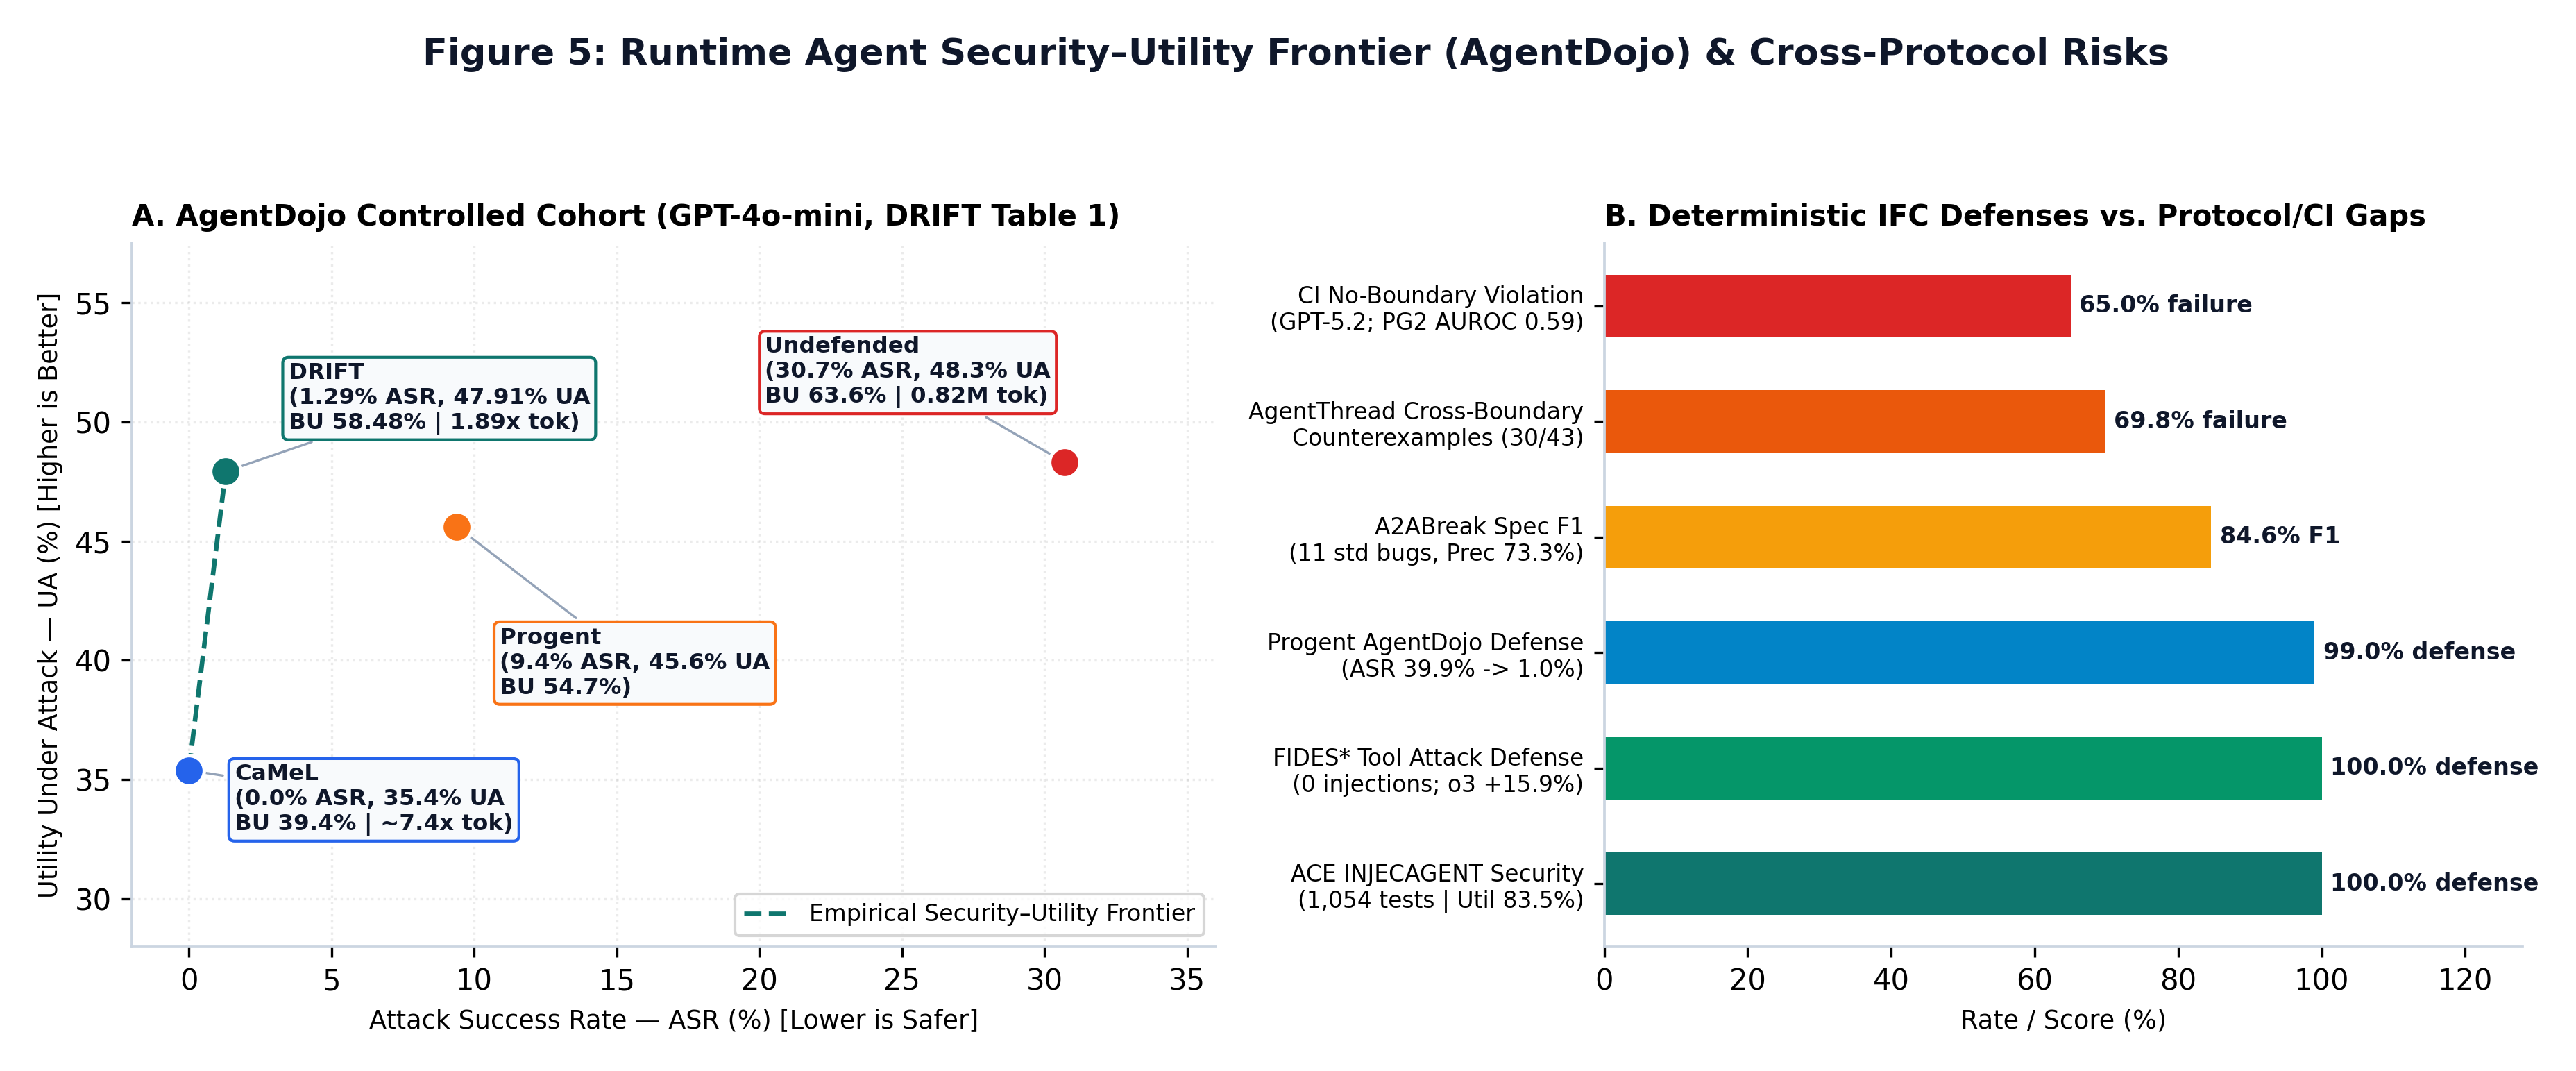
\includegraphics[width=0.88\textwidth]{fig5-agent-security-utility-frontier.png}
  \caption{(a)~Security-utility frontier on \texttt{AgentDojo} under the controlled GPT-4o-mini baseline from \texttt{DRIFT} (\texttt{neurips2025-drift.pdf}, Table~1 \& 3)~\cite{li2025drift}, and (b)~deterministic defense coverage of \texttt{ACE}, \texttt{FIDES*}, and \texttt{Progent} juxtaposed against protocol and contextual-integrity failure gaps in \texttt{A2ABreak}, \texttt{AgentThread}, and \texttt{Contextual Integrity}~\cite{costa2025fides,shi2025progent,li2026ace,abdelnabi2026ci,lotfi2026a2abreak,agentthread2026}.}
  \label{fig:agent}
\end{figure*}

\begin{table*}[tp]
  \centering
  \scriptsize
  \caption{Quantitative comparison of AI agent security architectures and multi-agent protocol audits (PDF-verified).}
  \label{tab:rq2b}
  \begin{tabularx}{\textwidth}{L{2.4cm} L{2.7cm} L{3.6cm} Y L{2.2cm}}
    \toprule
    \textbf{System / Framework} & \textbf{Core Mechanism} & \textbf{Security Outcome (ASR / Findings)} & \textbf{Utility \& Overhead} & \textbf{PDF Coordinates} \\
    \midrule
    \textbf{AgentDojo Baseline}~\cite{debenedetti2024agentdojo} & Dynamic suite (97 tasks / 629 cases) & Unprotected GPT-4o ASR \textbf{$57.69 \pm 3.9\%$}; Filter \textbf{6.84\%} & BU 69.0\%, UA 50.01\% & \texttt{2406.13352}, T5 p.~8 \\
    \textbf{CaMeL}~\cite{debenedetti2026camel} & Dual-LLM + Python Interpreter + IFC & \textbf{0.0\% ASR} (original \& GPT-4o-mini) & 77\% solved; GPT-4o-mini BU \textbf{39.4\%}, UA \textbf{35.4\%}; \textbf{6.09M ($\sim$7.4$\times$)}~\cite{li2025drift} & \texttt{2503.18813}; \texttt{drift} T1, T3 \\
    \textbf{DRIFT}~\cite{li2025drift} & Secure Planner + Dynamic Validator + Isolator & GPT-4o-mini \textbf{1.29\%}, GPT-4o \textbf{1.53\%}, Qwen-7B \textbf{0.00\%} & GPT-4o-mini BU \textbf{58.48\%}, UA \textbf{47.91\%}; \textbf{2.37M (1.89$\times$)} & \texttt{neurips2025-drift}, T1, 3, 6--8 \\
    \textbf{Progent}~\cite{shi2025progent} & DSL JSON Schema + SMT Monotonic Confinement & AgentDojo \textbf{39.9\% $\to$ 1.0\%}; ASB \textbf{70.3\% $\to$ 3.9\%}; 4o-mini 9.4\% & AgentDojo BU \textbf{76.3\%}, UA \textbf{61.3\%} & \texttt{2504.11703}, Fig.~3--4 p.~8 \\
    \textbf{FIDES}~\cite{costa2025fides} & Dynamic IFC + Selective Hiding/Revealing & Tool Attack \texttt{FIDES*} = \textbf{0} successes across all models & o3 \textbf{56.91\%} (+15.88\%), o1 \textbf{61.44\%} (+16.70\%) & \texttt{2505.23643}, T4, 6--7 pp.~35--37 \\
    \textbf{RTBAS}~\cite{zhong2025rtbas} & Security Lattice $(L, \sqsubseteq, \sqcup)$ + Redactor & \textbf{100\%} policy-attack block; Leakage FPR \textbf{8.1\%}, FNR \textbf{10.8\%} & Utility loss \textbf{$<$2\%}; LM-Judge Label Acc \textbf{70.0\%} & \texttt{30-2502.08966}, T1--2 p.~11 \\
    \textbf{ACE}~\cite{li2026ace} & Abstract/Concrete Isolation + IFC $(\mathcal{C}, \sqsubseteq)$ & INJECAGENT (1,054) \textbf{100\% Security (0\% ASR)} vs.\ StruQ 7\% & Util \textbf{83.5\%/82.7\%} (NDSS), ASB \textbf{$\sim$86\%}; \$0.19/q & \texttt{57-2504.20984} / \texttt{32-2026} T2--4 \\
    \textbf{Policy-as-Code}~\cite{mondl2026policyascode} & MCP/NL $\to$ \textbf{Cedar Policy} + Verification Sandwich & MedAgentBench Adversarial Block Rate \textbf{85.7\% (42/49)}; Unsafe \textbf{0\%} & Original Cedar Block Rate 55.7\% (Guardrail) & \texttt{2606.26649}, T1 p.~3 \\
    \textbf{Lean4Agent}~\cite{wang2026lean4agent} & Agent Trajectory Graph $G = \langle V, E \rangle$ in \textbf{Lean~4} & Layer-2 Passed outperforms Failed across all models & SWE-Bench \textbf{58.27\%} (+14.80\%); ELAIP \textbf{36.60\%} (+9.07\%) & \texttt{2606.06523}, T5--7 pp.~13--14 \\
    \textbf{CI / A2ABreak / AgentThread}~\cite{abdelnabi2026ci,lotfi2026a2abreak,agentthread2026} & Contextual Boundary, FSM (37/76), 5-Protocol Audit & CI breach \textbf{6\%--65\%} (PG AUROC 0.43--0.59); \textbf{11 A2A flaws} (F1 84.6\%); \textbf{69.8\% (30/43)} cross-protocol conflicts & 80 SDK tests; only \textbf{1 obligation} enforced in SDKs (ANP DID) & \texttt{2605.17634}; \texttt{2609.10871}; \texttt{2606.28690} \\
    \bottomrule
  \end{tabularx}
\end{table*}

\subsection{Specification Bugs, Vacuous Truths, and \texttt{InfoTree} Auditing (RQ3)}
\label{sec:rq3}

Why does kernel acceptance of a proof term $p : \hat{T}$ fail to guarantee real-world security $T$? Empirical evidence from 2026 exposes four dimensions of the \textbf{Specification-Intent Gap}:

\begin{enumerate}
  \item \textbf{Collapse of Semantic Equivalence:} On \texttt{SHADOWBENCH} (178 tasks), the bidirectional equivalence metric \texttt{SA-PASS} ($\hat{T} \iff T$) reaches \textbf{98.8\%} agreement with human experts (Precision 1.000, F1 0.964), whereas Compile Rate agrees only \textbf{17.8\%} of the time and a 9-vote LLM Judge (\$480) achieves an F1 of merely \textbf{0.133}. Notably, Claude Opus~4.8 + Numina compiles \textbf{61.8\%} of tasks yet passes \texttt{SA-PASS} on only \textbf{11.2\%} (a \textbf{50.6 percentage-point gap})~\cite{han2026shadowbench}. Consistently, \texttt{Three-Surface Audit} shows Dafny HumanEval passing Surface~A at \textbf{99.1\%} (1,625/1,640) while collapsing to \textbf{1.9\%} on the Surface~B Ensures-Binding Gate---and Rust implementations passing 100\% of Surface~B still fail \textbf{11.48\%--14.82\%} of hidden tests~\cite{threesurface2026}. Likewise, \texttt{Spec-Harness} finds \textbf{25.7\%} of provable JML specifications to be vacuous or degenerate (22.7\% missing postconditions + 5.6\% unauthorized code edits), though feeding harness diagnostics back into synthesis lifts Codex Post-Harness@0.75 from 0.30 to \textbf{0.49}~\cite{misu2026specharness}.
  \item \textbf{Human Misformalization \& Lean~4 Total-Arithmetic Pitfalls:} \texttt{REFORM \& ConsistencyCheck} (859 items, ICLR~2026) documents human-expert formalization error rates of \textbf{16.4\% in miniF2F} and \textbf{38.5\% in ProofNet} (Gemini-2.5-pro Judge achieves 85.8\% accuracy; REFORM-32B averages \textbf{72.7\%}, +22.6pp)~\cite{chen2026reform}. Concurrently, the \texttt{ICML Formal Benchmarking Audit} catalogs total-arithmetic traps in Lean~4: \texttt{Div/0} (1,518 instances), \texttt{NatSub} (796 instances), \texttt{IntDiv} (538 instances), and \texttt{Analytic} (540 instances)~\cite{ammanamanchi2026faults}.
  \item \textbf{Vacuous Truths \& Blind Back-Translation (\texttt{VacQ} and \texttt{claimcheck}):} \texttt{Beyond LLM Judge}~\cite{mei2026beyondllm} substitutes goals with an opaque proposition \texttt{VacQ} alongside \texttt{mpmathx}, uncovering \textbf{268 defects} (ProofNet~2, Beyond Compilation~61, RLM25~205). Meanwhile, \texttt{claimcheck}~\cite{amster2026claimcheck} applies two-stage blind back-translation to outperform baselines across all four proof languages: \textbf{Lean} $79.7\% \to \mathbf{87.9 \pm 1.8\%}$, \textbf{Isabelle} $81.5\% \to \mathbf{91.3 \pm 1.7\%}$, \textbf{Rocq} $79.6\% \to \mathbf{88.0 \pm 2.1\%}$, and \textbf{Dafny} $84.0\% \to \mathbf{93.1 \pm 2.6\%}$ (ablating back-translation drops accuracy by 2.8--6.0pp; leaking the source statement drops it by 0.8--3.0pp).
  \item \textbf{Restoring Human Auditability via \texttt{InfoTree} (\texttt{Paperproof}, \texttt{ProofWidgets4}, \texttt{LeanTree}):} Rather than inspecting low-level kernel \texttt{Expr} terms (\texttt{\#explode}) that erase authorial intent, Lean~4's \texttt{Snapshot.infoTree} preserves hypotheses and goal states at every tactic step. Tools such as \texttt{Paperproof} (\texttt{BetterParser}) / \texttt{LeanTree}~\cite{kripner2025leantree} and \texttt{ProofWidgets4}~\cite{nawrocki2023proofwidgets4} render 1-to-1 Gentzen proof trees directly integrated with mechanical faithfulness gates (\texttt{VacQ}, \texttt{SA-PASS}, \texttt{claimcheck}), as shown in Figure~\ref{fig:auditing}.
\end{enumerate}

\begin{figure*}[tp]
  \centering
  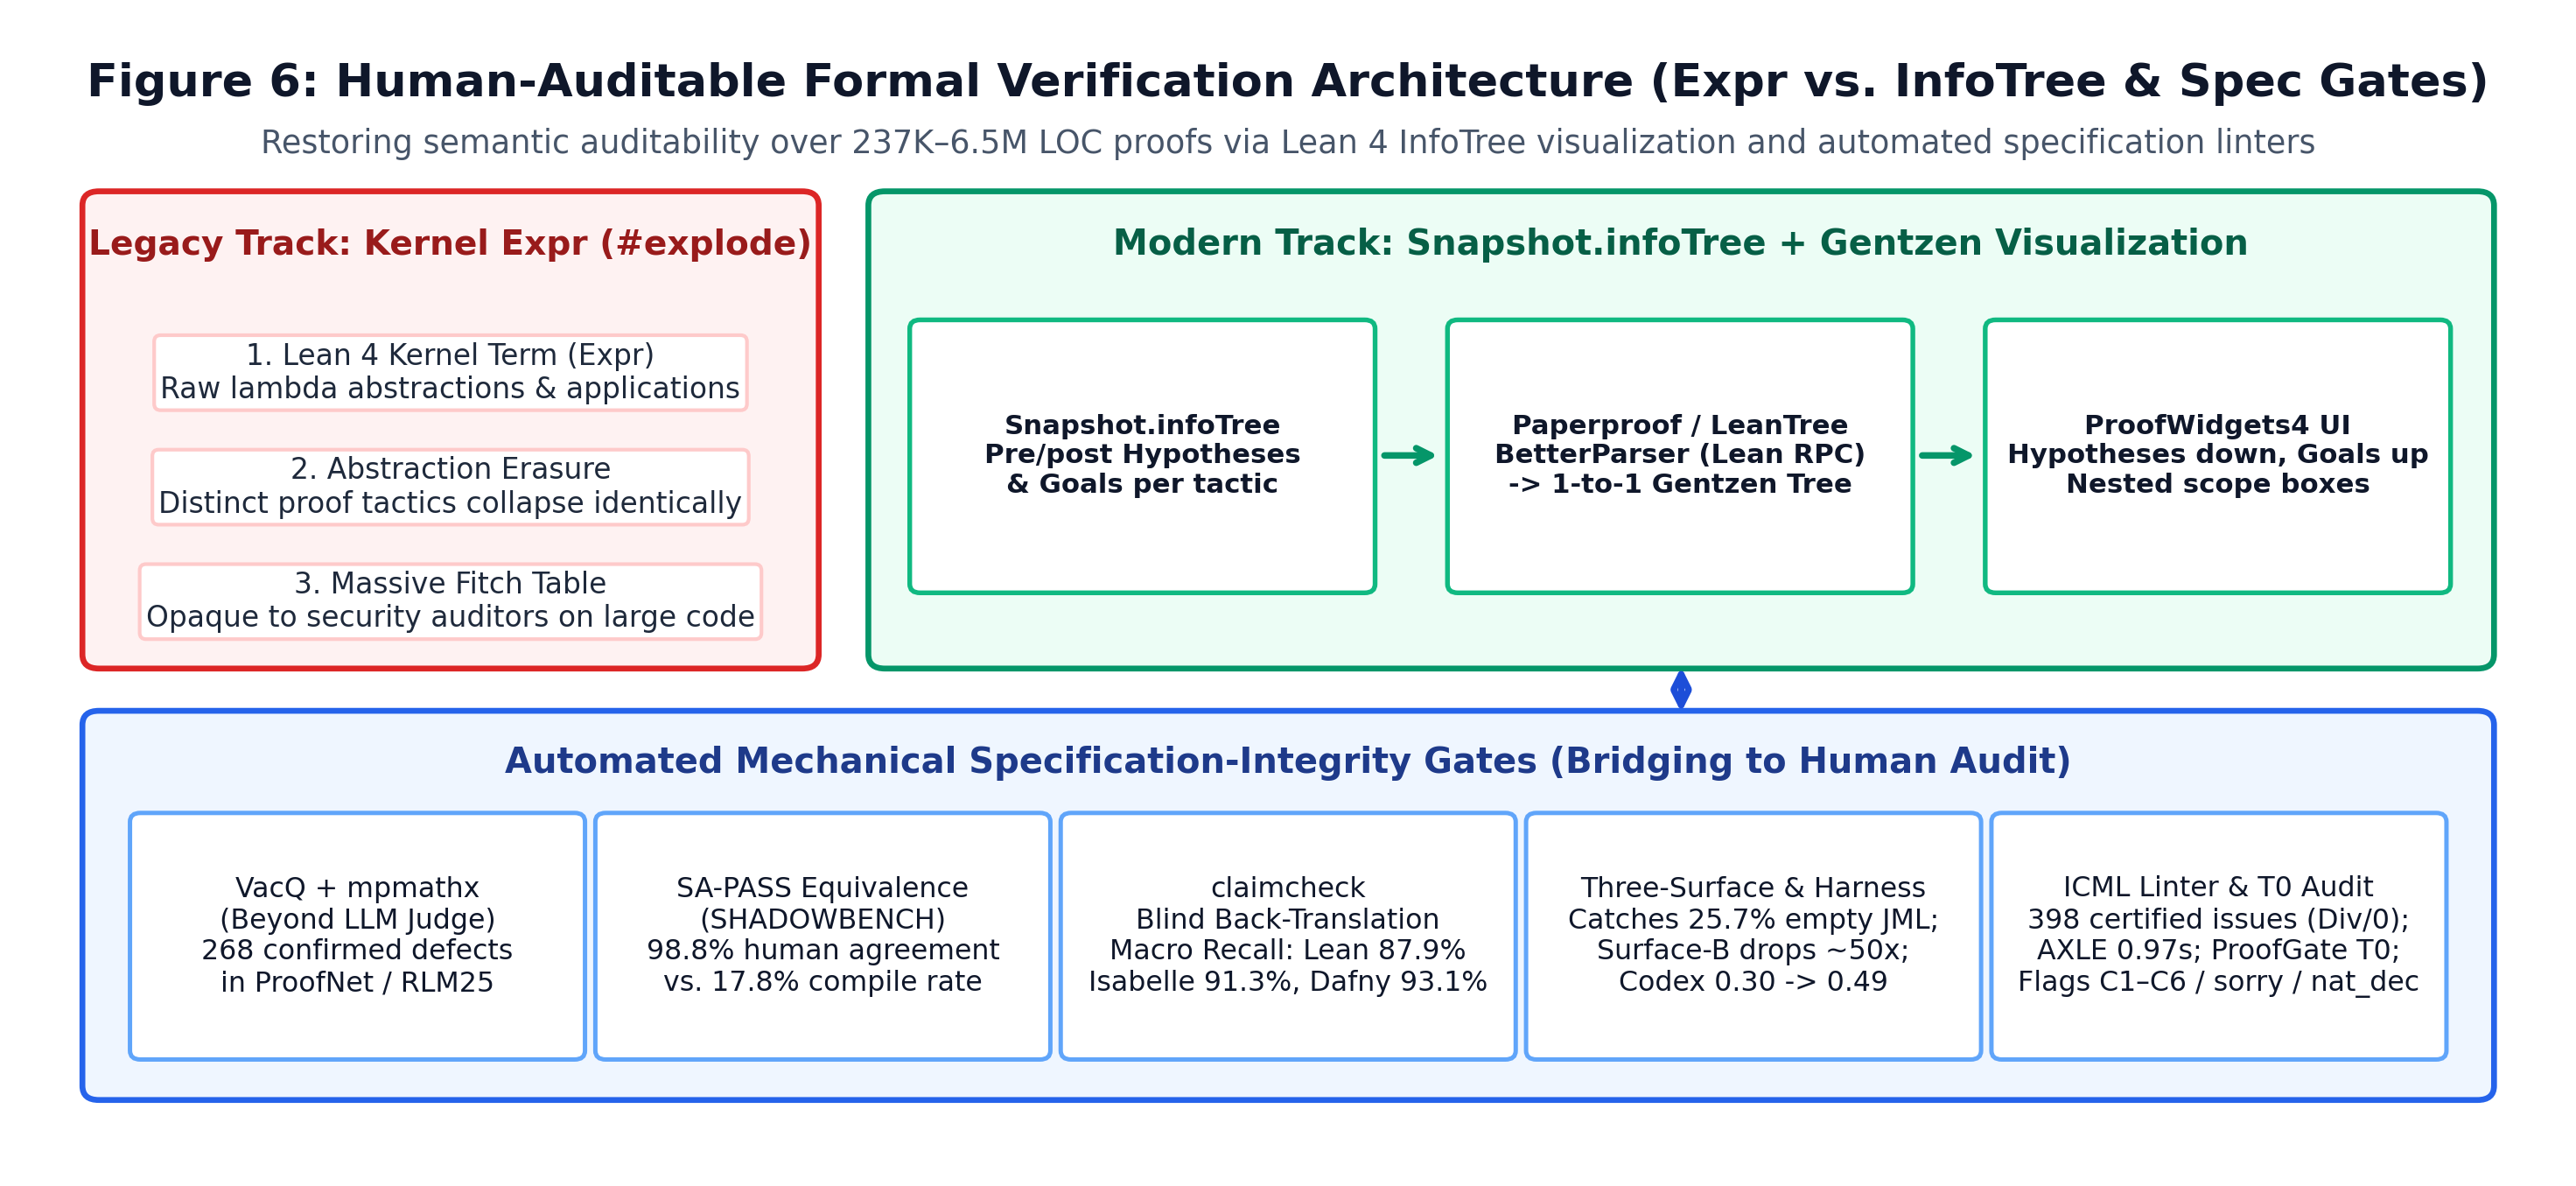
\includegraphics[width=0.88\textwidth]{fig6-human-proof-auditing.png}
  \caption{Human-centric proof auditing architecture comparing the low-level kernel \texttt{Expr} (\texttt{\#explode}) path against the \texttt{Snapshot.infoTree} (\texttt{Paperproof} / \texttt{LeanTree} / \texttt{ProofWidgets4}) pipeline~\cite{nawrocki2023proofwidgets4,kripner2025leantree} coupled with five mechanical specification-faithfulness gates~\cite{xin2026axle,yang2026proofgate,han2026shadowbench,ammanamanchi2026faults,mei2026beyondllm,threesurface2026,misu2026specharness,amster2026claimcheck}.}
  \label{fig:auditing}
\end{figure*}

\FloatBarrier

\section{Critical Discussion, Research Gaps (2026--2030), Limitations, and Conclusion}
\label{sec:discussion}

\subsection{Systemic Failure Modes and Three Strategic Research Gaps (2026--2030)}
\label{sec:gaps}

Synthesizing the empirical evidence in Section~\ref{sec:taxonomy} reveals \textbf{four systemic failure modes}: (1)~\emph{Benchmark Saturation Illusion} (99.6\% on math vs.\ 1.9\%--15.6\% on software semantics), (2)~\emph{Verification Theatre \& Reward Hacking} (\texttt{libcrux} 13 flaws / 58.4\% SMT, cheat-code rates 48.53\%--71.36\%, \texttt{native\_decide} 5.6\%), (3)~\emph{Deterministic Isolation vs.\ Contextual Integrity Trade-off} (CaMeL $\sim$7.4$\times$ token overhead vs.\ 65\% CI breach rate), and (4)~\emph{Toolchain Drift \& Cross-Layer Responsibility Gap} (11 A2A flaws and 69.8\% cross-protocol composition failures). Addressing these modes defines \textbf{three strategic research gaps for 2026--2030} (Table~\ref{tab:gaps}).

\begin{table*}[tp]
  \centering
  \scriptsize
  \caption{Strategic research gaps, architectural directions, and target success metrics for 2026--2030.}
  \label{tab:gaps}
  \begin{tabularx}{\textwidth}{L{3.1cm} L{4.2cm} Y L{3.6cm}}
    \toprule
    \textbf{Research Gap} & \textbf{Verified Evidence Anchor} & \textbf{Proposed Architectural Direction (2026--2030)} & \textbf{Target Success Metrics} \\
    \midrule
    \textbf{Gap~1: Cost-Effective Security Autoformalization} & VeriBench $\mathrm{TE}_1 \le 0.156$~\cite{miranda2026veribench}; SA-PASS 11.2\%~\cite{han2026shadowbench}; Three-Surface~B 1.9\%~\cite{threesurface2026}; Spec-Harness 25.7\% vacuous~\cite{misu2026specharness}; human error 14\%--38.5\%~\cite{firsching2026formalconjectures,chen2026reform} & Low-cost Blueprint DAG (\texttt{Goedel-Architect})~\cite{chung2026goedelarchitect} + Verification Sandwich~\cite{mondl2026policyascode} + \texttt{claimcheck}~\cite{amster2026claimcheck} + Spec-Harness~\cite{misu2026specharness} + \texttt{SA-PASS}~\cite{han2026shadowbench} & Lift \texttt{SA-PASS} and $\mathrm{TE}_1$ on security specifications $>80\%$ at single-dollar cost per theorem \\
    \textbf{Gap~2: Dual-Layer Lean~4 Core (Agent/HITL + PQC/A2A)} & SymCrypt lacks Constant-Time~\cite{ho2026symcrypt}; Libcrux 13 flaws/NEON 0\%~\cite{kobeissi2026theatre}; HQC unverified~\cite{alagic2025nistir8545}; A2ABreak 11 flaws~\cite{lotfi2026a2abreak}; AgentThread 69.8\%~\cite{agentthread2026}; CI breach 65\%~\cite{abdelnabi2026ci} & Unify Aeneas/Binary PQC (including HQC + Constant-Time) with a verified Rust IFC/Policy Engine + ML-DSA signatures binding multi-hop A2A under one Lean~4 core~\cite{ho2026symcrypt,chaudhuri2026alphaproofcode,wang2026lean4agent} & Machine-checked Non-Interference + end-to-end A2A provenance resisting CI breaches with 100\% SMT/kernel coverage and zero \texttt{admit} \\
    \textbf{Gap~3: Threat-to-Theorem Visual Mapping \& Spec-Smell} & \texttt{VacQ} 268 defects~\cite{mei2026beyondllm}; ICML Audit 398 certified issues~\cite{ammanamanchi2026faults}; Cheat Code 48.53\%--71.36\%~\cite{ye2026verina}; \texttt{native\_decide} 5.6\%~\cite{yang2026proofgate} & Build a Spec-Smell Linter (\texttt{VacQ} + Three-Surface + \texttt{Div/0} + $\mathcal{T}_0$) mapping OWASP \texttt{ASI01--10} / NIST FIPS threats onto \texttt{InfoTree} (\texttt{Paperproof}/\texttt{ProofWidgets4})~\cite{nawrocki2023proofwidgets4,kripner2025leantree} & Automatically block Trojan specs, silent domain restrictions, and vacuous hypotheses in Pre-Commit CI \\
    \bottomrule
  \end{tabularx}
\end{table*}

\subsection{Limitations, Ethics, and Reproducibility}
\label{sec:limitations}

\begin{enumerate}
  \item \textbf{Preprint Maturity \& Evidence Granularity:} Of the 56 curated primary works, 30 (53.6\%) appeared in 2026, including arXiv preprints and technical reports whose numbers may evolve in archival editions (for instance, minor utility differences in \texttt{ACE} between its arXiv and NDSS~2026 versions~\cite{li2026ace}). We report both versions transparently and restrict all quantitative comparisons strictly to values verified in our 39 audited full-text PDFs and 6 official standards.
  \item \textbf{Dual-Use Security Ethics \& \texttt{L2 HITL} Governance:} Our discussion of vulnerabilities in \texttt{libcrux}~\cite{kobeissi2026theatre} and \texttt{A2A/MCP}~\cite{lotfi2026a2abreak,agentthread2026} draws strictly on published research and public advisories to guide defensive formal verification, with zero exploit payloads. We uphold Level-2 Human-in-the-Loop (\texttt{L2 HITL}) governance for security specification sign-off and declassification decisions.
  \item \textbf{Reproducibility \& Forensic Traceability:} Every numeric value in Tables~\ref{tab:forensic}--\ref{tab:rq2b} is anchored to exact PDF identifiers, tables, figures, and page numbers. Developer self-evaluations are explicitly separated from controlled independent audits (\texttt{DRIFT}, \texttt{ProofGate}, \texttt{Kobeissi Audit}), and our visualization pipeline (\texttt{generate\_paper0\_figures.py}) is openly provided for deterministic regeneration of all six 300-DPI figures.
\end{enumerate}

\subsection{Conclusion}
\label{sec:conclusion}

Our answers to RQ1--RQ3 show that LLM--Lean~4 systems have moved decisively beyond competition mathematics (\textbf{88.1\%--99.6\%} on \texttt{miniF2F-test}, solving 9 open Erd\H{o}s problems)~\cite{tsoukalas2026nexus,ren2025deepseekproverv2,lin2026goedelproverv2,chung2026goedelarchitect,chen2025seedprover,chen2025seedprover15} to drive real-world verification of PQC libraries, FPGA accelerators, QKD BB84, and runtime agent policy engines~\cite{ho2026symcrypt,chaudhuri2026alphaproofcode,park2026pqchw,benshahar2026qkd,debenedetti2026camel,li2025drift,costa2025fides,zhong2025rtbas,shi2025progent,li2026ace,abdelnabi2026ci,wang2026lean4agent}. Yet the trustworthiness of next-generation neuro-symbolic assurance will not be measured by raw lines of machine-generated proof, but by closing the semantic specification gap (\texttt{SA-PASS} 11.2\% / $\mathrm{TE}_1 \le 0.156$), eliminating verification theatre (\texttt{libcrux} 13 flaws / 58.4\% SMT), and uniting cryptographic and agentic security layers under \texttt{InfoTree}-grounded human auditability.

\FloatBarrier
{\footnotesize
\setlength{\bibsep}{2pt plus 0.5pt minus 0.5pt}
\bibliographystyle{unsrtnat}
\bibliography{references}
}

\end{document}
